\documentclass[11pt]{article}
\usepackage[a4paper,margin=19mm]{geometry}
\usepackage[no-math]{fontspec}
\setmainfont{Latin Modern Roman}[SmallCapsFont=Latin Modern Roman Caps]
\usepackage{amsmath,amssymb,amsthm,mathtools,amscd,verbatim,xcolor,graphicx,hyperref}
\hypersetup{hidelinks}
\numberwithin{equation}{section}
\newtheorem{theorem}{Theorem}[section]
\newtheorem{lemma}[theorem]{Lemma}
\newtheorem{proposition}[theorem]{Proposition}
\newtheorem{corollary}[theorem]{Corollary}
\newtheorem{claim}[theorem]{Claim}
\newtheorem{fact}[theorem]{Fact}
\newtheorem{conjecture}[theorem]{Conjecture}
\theoremstyle{definition}
\newtheorem{definition}[theorem]{Definition}
\newtheorem{example}[theorem]{Example}
\newtheorem{remark}[theorem]{Remark}
\newtheorem{question}[theorem]{Question}
\theoremstyle{plain}
\newcommand{\C}{\mathbb C}
\newcommand{\R}{\mathbb R}
\newcommand{\Q}{\mathbb Q}
\newcommand{\Z}{\mathbb Z}
\newcommand{\N}{\mathbb N}
\newcommand{\eee}{\mathrm e}
\newcommand{\cclass}[1]{\textsf{#1}}
\newcommand{\cproblem}[1]{\textsc{#1}}
\newcommand{\ie}{i.\,e.}
\newcommand{\Ie}{I.\,e.}
\newcommand{\eg}{e.\,g.}
\newcommand{\Eg}{E.\,g.}
\newcommand{\phd}{Ph.\,D.}
\newcommand{\msc}{M.\,S.}
\newcommand{\bsc}{B.\,S.}
\newcommand{\expref}[2]{\hyperref[#2]{#1~\ref{#2}}}
\newcommand{\expeqref}[2]{\hyperref[#2]{#1~\eqref{#2}}}
\newcommand{\exprefsilent}[2]{\hyperref[#2]{#1}}
\newcommand{\epfmtdoi}[1]{\href{https://doi.org/#1}{doi:#1}}
\emergencystretch=3em
\usepackage{etoolbox,bm}
\newcommand{\epfmt}[2]{\begingroup\def\TocNativeBibResult{\PackageError{toc-native-compat}{Unsupported bibliography type/record #1/#2}{Only exact source-observed finite records are allowed.}}\ifstrequal{#1}{arxiv}{\ifstrequal{#2}{1210.0049}{\def\TocNativeBibResult{\href{http://arxiv.org/abs/1210.0049}{arXiv:#2}}}{}}{}\ifstrequal{#1}{arxiv}{\ifstrequal{#2}{1610.01199}{\def\TocNativeBibResult{\href{http://arxiv.org/abs/1610.01199}{arXiv:#2}}}{}}{}\ifstrequal{#1}{arxiv}{\ifstrequal{#2}{1806.04256}{\def\TocNativeBibResult{\href{http://arxiv.org/abs/1806.04256}{arXiv:#2}}}{}}{}\ifstrequal{#1}{arxiv}{\ifstrequal{#2}{1912.04524}{\def\TocNativeBibResult{\href{http://arxiv.org/abs/1912.04524}{arXiv:#2}}}{}}{}\ifstrequal{#1}{arxiv}{\ifstrequal{#2}{2002.07208}{\def\TocNativeBibResult{\href{http://arxiv.org/abs/2002.07208}{arXiv:#2}}}{}}{}\ifstrequal{#1}{arxiv}{\ifstrequal{#2}{2101.01151}{\def\TocNativeBibResult{\href{http://arxiv.org/abs/2101.01151}{arXiv:#2}}}{}}{}\ifstrequal{#1}{eccc}{\ifstrequal{#2}{TR00-004}{\def\TocNativeBibResult{\href{https://eccc.weizmann.ac.il/report/2000/004}{ECCC:#2}}}{}}{}\ifstrequal{#1}{eccc}{\ifstrequal{#2}{TR09-070}{\def\TocNativeBibResult{\href{https://eccc.weizmann.ac.il/report/2009/070}{ECCC:#2}}}{}}{}\ifstrequal{#1}{eccc}{\ifstrequal{#2}{TR10-088}{\def\TocNativeBibResult{\href{https://eccc.weizmann.ac.il/report/2010/088}{ECCC:#2}}}{}}{}\ifstrequal{#1}{eccc}{\ifstrequal{#2}{TR12-123}{\def\TocNativeBibResult{\href{https://eccc.weizmann.ac.il/report/2012/123}{ECCC:#2}}}{}}{}\ifstrequal{#1}{eccc}{\ifstrequal{#2}{TR17-161}{\def\TocNativeBibResult{\href{https://eccc.weizmann.ac.il/report/2017/161}{ECCC:#2}}}{}}{}\ifstrequal{#1}{eccc}{\ifstrequal{#2}{TR18-063}{\def\TocNativeBibResult{\href{https://eccc.weizmann.ac.il/report/2018/063}{ECCC:#2}}}{}}{}\ifstrequal{#1}{eccc}{\ifstrequal{#2}{TR18-112}{\def\TocNativeBibResult{\href{https://eccc.weizmann.ac.il/report/2018/112}{ECCC:#2}}}{}}{}\ifstrequal{#1}{eccc}{\ifstrequal{#2}{TR20-016}{\def\TocNativeBibResult{\href{https://eccc.weizmann.ac.il/report/2020/016}{ECCC:#2}}}{}}{}\ifstrequal{#1}{eccc}{\ifstrequal{#2}{TR20-069}{\def\TocNativeBibResult{\href{https://eccc.weizmann.ac.il/report/2020/069}{ECCC:#2}}}{}}{}\ifstrequal{#1}{eccc}{\ifstrequal{#2}{TR21-019}{\def\TocNativeBibResult{\href{https://eccc.weizmann.ac.il/report/2021/019}{ECCC:#2}}}{}}{}\ifstrequal{#1}{eccc}{\ifstrequal{#2}{TR21-020}{\def\TocNativeBibResult{\href{https://eccc.weizmann.ac.il/report/2021/020}{ECCC:#2}}}{}}{}\ifstrequal{#1}{eccc}{\ifstrequal{#2}{TR21-048}{\def\TocNativeBibResult{\href{https://eccc.weizmann.ac.il/report/2021/048}{ECCC:#2}}}{}}{}\ifstrequal{#1}{eccc}{\ifstrequal{#2}{TR94-002}{\def\TocNativeBibResult{\href{https://eccc.weizmann.ac.il/report/1994/002}{ECCC:#2}}}{}}{}\ifstrequal{#1}{eccc}{\ifstrequal{#2}{TR97-011}{\def\TocNativeBibResult{\href{https://eccc.weizmann.ac.il/report/1997/011}{ECCC:#2}}}{}}{}\TocNativeBibResult\endgroup}

%% Theory of Computing
%% File: v018a021.tex
%% Publication date: September 20, 2022
%% Authors: Kuan Cheng and William M. Hoza

%

%
%
%
%

%

%
%
%
%
%
%
%
%
	%
		%
		%
	%
	%
	%
%
%
%
%
%
%
%
%

%




%
%
%
   %

%
%
%
%
%
%
%
%
%
%
%
%
%
%
%
%
%
%
%
%
%
%
%
%
%
%
%
%
%

%
%
   %

%
%
%
%
%
%
\usepackage{tikz}
%

%
%
%

\DeclareMathOperator*{\ExpVal}{\mathbb{E}}


\begin{document}
\begin{center}{\Large Stable item 968: Conditional deterministic small-space acceptance-probability estimation from hitting sets for wider branching programs}\end{center}
\paragraph{Source and attribution.}
Kuan Cheng and William M. Hoza, \emph{Hitting Sets Give Two-Sided Derandomization of Small Space}. Theory of Computing 18 (2022), Article 21, publisher source publication September 20, 2022; DOI 10.4086/toc.2022.v018a021. \href{https://theoryofcomputing.org/articles/v018a021/}{Publisher article}. Original human statement/proof/context: \href{https://creativecommons.org/licenses/by/3.0/}{CC BY3.0}.
\paragraph{Selected problem and source scope.}
Prove only the authors' Theorem 2.1 (original label \detokenize{thm:HSGDerandROBP}) below. The full original mathematical article and bibliography are preserved as conservative closed context. The assumed hitting set is for the source's explicitly enlarged width and length, with the uniform family-space interpretation at original line 492. The author sample-existence proof explicitly considers sufficiently large n (line 538); preserve that source asymptotic convention without promoting new finite-case claims. The separate black-box sampler branch is unqualified context due to its documented prefix-index question. Other equivalent formulations, consequences and supporting lemmas are uncounted.
\paragraph{Difficulty (editorial): H3.}
The selected two-sided derandomization builds a wider branching program that verifies a full table of sampled vertex-reachability probabilities, rather than merely searching a hitting set for an accepting input. Its complete author core proves that a source-local consistency test propagates bounded total layer error while accepting a sample table guaranteed by the assumed hitting set. The construction also gives an explicit repeated-read small-space implementation with exact dyadic counters, so its main obstacle is a nonroutine uniform verification-and-estimation reduction rather than routine concentration or a restated L=BPL consequence.
\paragraph{Editorial source boundary.}
Author mathematical TeX and ordering are unchanged. Only journal front matter is replaced by this wrapper; exact authored macros are flattened and separately preserved, and finite source-observed display aliases are defined in the standalone preamble. The original inline TikZ implication diagram remains fully native and editable, with literal authored picture code. Canonical DOI follows the observed official landing citation; the literal native punctuation discrepancy is retained in original source/context metadata. No generated proof, mathematical repair or independent mathematical refereeing is supplied. 
\clearpage

%
%
%
	 	
\section{Introduction} \label{sec:intro}
Suppose some decision problem can be solved by an efficient randomized algorithm. That's good, but an efficient deterministic algorithm would be even better. We would therefore like to deterministically analyze the acceptance probability of the randomized algorithm on a given input. An ambitious approach to derandomization is to try to design a suitable \emph{pseudorandom generator} (PRG).
\begin{definition}
Let $\mathcal{F}$ be a class of functions $f \colon \{0, 1\}^n \to \{0, 1\}$. An \emph{$\epsilon$-PRG} for $\mathcal{F}$ is a function $G \colon \{0, 1\}^s \to \{0, 1\}^n$ such that for every $f \in \mathcal{F}$,
$
\left|\ExpVal[f] - \ExpVal_{X \in \{0, 1\}^s}[f(G(X))]\right| \leq \epsilon.
$
\end{definition}
Let $n$ be the number of random bits used by the randomized algorithm, and ensure that $\mathcal{F}$ can compute the action of the randomized algorithm on its random bits. By iterating over all ``seeds'' $x \in \{0, 1\}^s$ and plugging $G(x)$ into the randomized algorithm, we can get an estimate of its acceptance probability with additive error at most $\epsilon$.

Unfortunately, designing efficient PRGs has proved to be extremely difficult. Constructing a \emph{hitting set} is sometimes less difficult.
\begin{definition}
Let $\mathcal{F}$ be a class of functions $f \colon \{0, 1\}^n \to \{0, 1\}$. An \emph{$\epsilon$-hitting set} for $\mathcal{F}$ is a set $H \subseteq \{0, 1\}^n$ such that for every $f \in \mathcal{F}$ with $\ExpVal[f] \geq \epsilon$, there is some $x \in H$ such that $f(x) = 1$.
\end{definition}
The image of any $\epsilon$-PRG is clearly an $\epsilon'$-hitting set for every $\epsilon' > \epsilon$. By iterating over all strings in an $\epsilon$-hitting set, we can at least distinguish acceptance probability $0$ from acceptance probability $\geq \epsilon$. This is already sufficient for derandomizing some algorithms (namely, those with ``one-sided error''). In this paper, we investigate the possibility of using a hitting set in a nontrivial way to obtain an estimate of the acceptance probability with a small additive error, just like what a PRG would have provided.

This possibility was previously studied in the context of derandomizing time-bounded algorithms. Several proofs have been discovered showing that if there is a polynomial-time hitting set for size-$n$ circuits, then $\mathbf{P} = \mathbf{BPP}$ \cite{ACR98,BF99,ACRT99,GVW11}. In \expref{Section}{sec:bpp} we provide yet another proof of this theorem; our short proof is arguably simpler than all previous proofs. However, the focus of our paper is derandomizing space-bounded algorithms.

\subsection{Derandomizing log-space algorithms}

The behavior of a small-space algorithm as a function of its random bits can be modeled by a \emph{read-once\footnote{Because space-bounded algorithms only have read-once access to their random bits, it does not seem possible to adapt the existing derandomizations of $\mathbf{BPP}$ using a hitting set to the $\mathbf{BPL}$ case.} branching program} (ROBP). A width-$w$ length-$n$ ROBP is a directed graph consisting of $n + 1$ layers with $w$ vertices per layer. There is a designated ``start vertex'' $v_{\text{start}}$ in the first layer. Every vertex not in the last layer has two outgoing edges labeled $0$ and $1$ leading to the next layer. An $n$-bit input string naturally identifies a path through the graph by reading from left to right. The program accepts or rejects this string depending on whether the path ends at the designated ``accept vertex'' $v_{\text{acc}}$ in the last layer.

Recall that $\mathbf{BPL}$ and $\mathbf{RL}$ are the classes of languages that can be decided by randomized log-space algorithms that always halt with two-sided and one-sided error respectively. A log-space hitting set\footnote{When we say ``a log-space hitting set,'' we mean a family of hitting sets $H_n \subseteq \{0, 1\}^n$ such that given input $n \in \N$, the set $H_n$ can be enumerated in space $O(\log n)$. For such a family, $|H_n| \leq \text{poly}(n)$.} for polynomial-width ROBPs would immediately imply $\mathbf{L} = \mathbf{RL}$. For our first result, we show that such a hitting set would also imply $\mathbf{L}= \mathbf{BPL}$.

\begin{theorem} \label{thm:poly-width-main}
Assume that for every $n \in \N$, there is a $\frac{1}{2}$-hitting set for width-$n$, length-$n$ ROBPs that can be computed in space $O(\log n)$. Then $\mathbf{L} = \mathbf{BPL}$.
\end{theorem}

\subsection{Motivation: Recent work on hitting sets}

\expref{Theorem}{thm:poly-width-main} is especially interesting in light of recent constructions of improved hitting sets for ROBPs \cite{BCG20, HZ20, CL20}. The best PRG known for polynomial-width ROBPs is still Nisan's PRG \cite{Nis92}, which has seed length
$$
O(\log^2 n + \log n \log(1/\epsilon))\,.
$$
Until recently, Nisan's PRG also provided the best hitting set for polynomial-width ROBPs. Using sophisticated and novel techniques, Braverman, Cohen, and Garg obtained a hitting set with space complexity
$$
\widetilde{O}(\log^2 n + \log(1/\epsilon))\,,
$$
which is an improvement when $\epsilon$ is very small \cite{BCG20}.

Actually, Braverman, Cohen, and Garg constructed something better than a hitting set, called a \emph{weighted pseudorandom generator} (WPRG) or alternatively a \emph{pseudorandom pseudodistribution generator}.
\begin{definition}[\cite{BCG20}]
Let $\mathcal{F}$ be a class of functions $f \colon \{0, 1\}^n \to \{0, 1\}$. An \emph{$\epsilon$-WPRG} for $\mathcal{F}$ is a pair $(G, \rho)$, where $G \colon \{0, 1\}^s \to \{0, 1\}^n$ and $\rho \colon \{0, 1\}^s \to \R$, such that for every $f \in \mathcal{F}$,
\[
\left|\ExpVal[f] - \ExpVal_{X \in \{0, 1\}^s}[f(G(X)) \cdot \rho(X)]\right| \leq \epsilon\,.
\]
\end{definition}
A WPRG can be used to estimate $\ExpVal[f]$ to within $\pm \epsilon$, provided that $G$ and $\rho$ can both be computed efficiently. The concept of a WPRG generalizes the concept of a PRG, which is the special case $\rho(x) \equiv 1$. 
In turn, if $(G, \rho)$ is an $\epsilon$-WPRG, then the image of $G$ is an $\epsilon'$-hitting set for every $\epsilon' > \epsilon$. So a WPRG is \emph{intermediate} between a hitting set and a genuine PRG.

After Braverman, Cohen, and Garg's work \cite{BCG20}, Hoza and Zuckerman gave a simpler construction of an $\epsilon$-hitting set for polynomial-width ROBPs, with the slightly improved space complexity $O(\log^2 n + \log(1/\epsilon))$ \cite{HZ20}. Their construction is weaker in that it does not provide a WPRG. \expref{Theorem}{thm:poly-width-main} bridges the gap between the two concepts somewhat: by \expref{Theorem}{thm:poly-width-main}, any generic hitting set can be used for two-sided derandomization, which was the main strength of a WPRG over a hitting set in the first place.

(Independently of our work, Chattopadhyay and Liao gave an improved WPRG construction with seed length $\widetilde{O}(\log^2 n) + O(\log(1/\epsilon))$~\cite{CL20}. Further WPRG constructions were devised after the preliminary version of our work~\cite{conf-version} appeared, leading to a seed length of $O(\log^2 n + \log(1/\epsilon))$~\cite{CDRSTS21,PV21,Hoz21}, which matches the parameters of Hoza and Zuckerman's hitting set for polynomial-width ROBPs~\cite{HZ20}.)

\subsection{The constant-width setting}

However, there is a weakness of \expref{Theorem}{thm:poly-width-main}. A PRG or a WPRG would provide a \emph{black-box} derandomization, whereas the algorithm of \expref{Theorem}{thm:poly-width-main} is not black-box. This weakness is especially acute when we consider the constant-width case. Given a constant-width ROBP $f$ directly as input, it is trivial to compute $\ExpVal[f]$ with high accuracy, so the algorithm of \expref{Theorem}{thm:poly-width-main} is meaningless. Nevertheless, constant-width ROBPs can compute many interesting functions, and it is a major open challenge to design improved PRGs, WPRGs, or hitting sets for constant-width ROBPs. (For width $2$, optimal PRGs are known \cite{BDVY13}. For width $3$, the current best PRG has seed length $\widetilde{O}(\log n \log(1/\epsilon))$ \cite{MRT19}. The best hitting sets for width $3$ are superior, with space complexity $\widetilde{O}(\log(n/\epsilon))$ for small $\epsilon$ \cite{GMRTV12} or $O(\log n)$ for large enough $\epsilon$ \cite{SZ21}. For width $4$, the state of the art is simply the best results for polynomial-width ROBPs mentioned above~\cite{Nis92,HZ20,Hoz21}.)

To address this weakness of \expref{Theorem}{thm:poly-width-main}, we abstract the ``black-box'' feature of PRGs and WPRGs in the following definition.

\begin{definition}
Let $\mathcal{F}$ be a class of functions $f \colon \{0, 1\}^n \to \{0, 1\}$. A \emph{deterministic $\epsilon$-sampler} for $\mathcal{F}$ is a deterministic oracle algorithm $A$ that outputs a real number such that for every $f \in \mathcal{F}$,
$$
|A^f - \ExpVal[f]| \leq \epsilon\,.
$$
\end{definition}

The concept of a deterministic sampler generalizes that of a WPRG, because given a WPRG $(G, \rho)$ with seed length $s$, one can set $A^f = 2^{-s} \sum_x f(x) \rho(x)$. In the other direction, deterministic samplers imply hitting sets.

\begin{proposition}
Identify $0$ with the constant $0$ function on $\{0, 1\}^n$, and assume $0 \in \mathcal{F}$. Let $A$ be a deterministic $\epsilon$-sampler for $\mathcal{F}$, and let $H \subseteq \{0, 1\}^n$ be the set of points where $A^0$ queries its oracle. Then for every $\epsilon' > 2\epsilon$, $H$ is an $\epsilon'$-hitting set for $\mathcal{F}$.
\end{proposition}

\begin{proof}
Let $f \in \mathcal{F}$ satisfy $\ExpVal[f] > 2\epsilon$. Since $|A^0 - 0| \leq \epsilon$ and $|A^f - \ExpVal[f]| \leq \epsilon$, $A^0 \neq A^f$. Therefore, $A^f$ must query $f$ at some point $x \in f^{-1}(1)$. The \emph{first} such query must be at a point $x \in H$.
\end{proof}

The deterministic sampler model captures some prior derandomization algorithms. In particular, all known derandomizations of $\mathbf{BPP}$ using a hitting set~\cite{ACR98,BF99,ACRT99,GVW11}, including our new derandomization in \expref{Section}{sec:bpp}, can be interpreted as constructing deterministic samplers for circuits. For our second result, we prove the analogous reduction for constant-width ROBPs, \ie, we show that one can generically ``upgrade'' log-space hitting sets for such programs into log-space deterministic samplers. (See \expref{Figure}{fig:implications}.)


\begin{figure}[h]
\begin{center}

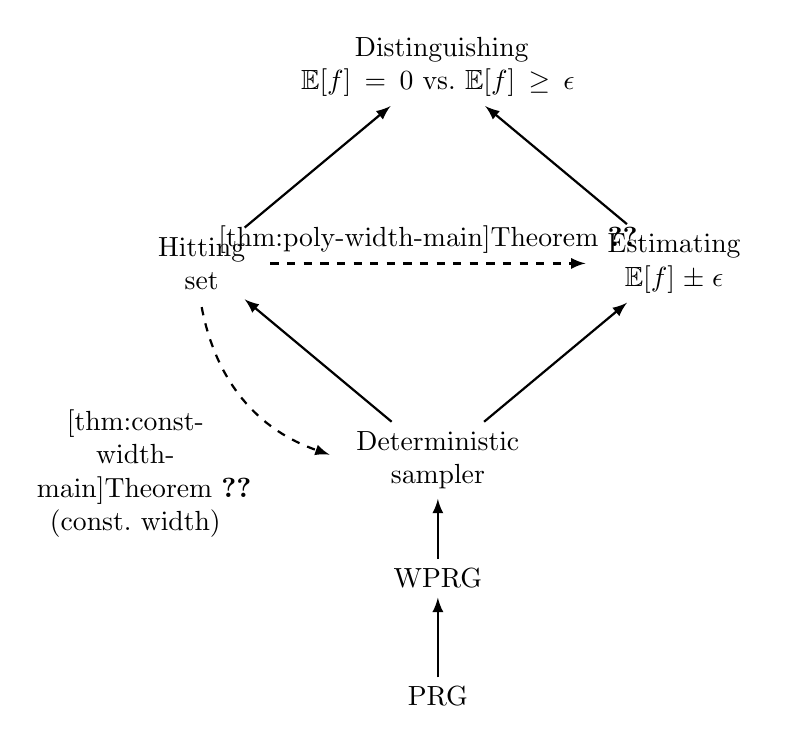
\begin{tikzpicture}
\node (v1) at (0,-2.5) {PRG};
\node (v2) at (0,-1) {WPRG};
\node[text width=2.5cm, align=center] (v3) at (0,0.5) {Deterministic sampler};
\node[text width=1.5cm, align=center] (v4) at (-3,3) {Hitting set};
\draw[->, thick, >=latex]  (v1) edge (v2);
\draw [->, thick, >=latex] (v2) edge (v3);
\draw [->, thick, >=latex] (v3) edge (v4);
\node[text width=2cm, align=center] (v5) at (3,3) {Estimating $\ExpVal[f] \pm \epsilon$};
\draw [->, thick, >=latex] (v3) edge (v5);
\draw [->, thick, dashed, >=latex] (v4) edge node[above] {\expref{Theorem}{thm:poly-width-main}} (v5);
\draw [->, thick, dashed, >=latex, bend right] ([yshift=-0.1cm]v4.south) to node[below left, text width=2.5cm, align=center] {\expref{Theorem}{thm:const-width-main} (const.\ width)} (v3);
%
\node[text width=4.5cm, align=center] (v6) at (0,5.5) {\; \; \; Distinguishing \; \; \; $\ExpVal[f] = 0$ vs.\ $\ExpVal[f] \geq \epsilon$}; 
%
\draw [->, thick, >=latex] (v4) edge (v6);
\draw [->, thick, >=latex] (v5) edge (v6);
\end{tikzpicture}
\end{center}

\caption{The relationships between different derandomization goals. The solid arrows are implications that are immediate from the definitions and hold for essentially any class $\mathcal{F}$ (possibly with some loss in $\epsilon$). The dashed arrows are theorems in this paper, holding for ROBPs specifically.} \label{fig:implications}
\end{figure}

\begin{theorem} \label{thm:const-width-main}
Assume that for every constant $w$, for all $n \in \N$, there is a $\frac{1}{2}$-hitting set for width-$w$ length-$n$ ROBPs that can be computed in space $O(\log n)$. Then for every constant $w$, for all $n \in \N$ and all $\epsilon > 0$, there is a deterministic $\epsilon$-sampler for width-$w$ length-$n$ ROBPs that runs in space $O(\log(n/\epsilon))$.
\end{theorem}

More generally, given a $\frac{1}{2}$-hitting set for width-$w'$ length-$n'$ ROBPs for suitable values $w' = O(w^2)$ and $n' = O(n^2/\epsilon)$, we show how to construct a deterministic $\epsilon$-sampler for width-$w$ length-$n$ ROBPs. If the hitting set has space complexity $s$, then our deterministic sampler has space complexity $O(s + w \log(n/\epsilon))$. See \expref{Theorem}{thm:const-width-reduction} and \expref{Corollary}{cor:const-width-main-generalization}.

The proof of \expref{Theorem}{thm:const-width-main} uses different techniques than that of \expref{Theorem}{thm:poly-width-main}. Because of the factor of $w$ in our deterministic sampler's space complexity, our sampler becomes meaningless when $w$ is large. Thus, \expref{Theorem}{thm:poly-width-main} and \expref{Theorem}{thm:const-width-main} are incomparable.

We also obtain a new \emph{unconditional} deterministic sampler. When $\epsilon$ is moderate, the best deterministic sampler for constant-width ROBPs is simply from Nisan's PRG \cite{Nis92}, which gives a sampler with space complexity $O(\log^2 n + \log n \log(1/\epsilon))$. When $\epsilon$ is small, using prior work, the best deterministic sampler for constant-width ROBPs was from Braverman, Cohen, and Garg's WPRG \cite{BCG20} (space complexity $\widetilde{O}(\log^2 n + \log(1/\epsilon))$). The concurrent work by Chattopadhyay and Liao \cite{CL20} gives a slightly better WPRG, and hence a slightly better deterministic sampler (space complexity $\widetilde{O}(\log^2 n) + O(\log(1/\epsilon))$). By applying the reduction underlying \expref{Theorem}{thm:const-width-main} to the hitting set of Hoza and Zuckerman \cite{HZ20}, we achieve a slightly better bound.

\begin{theorem}[Unconditional sampler] \label{thm:hz-sampler}
For every constant $w$, for all $n \in \N$ and all $\epsilon > 0$, there is a deterministic $\epsilon$-sampler for width-$w$ length-$n$ ROBPs running in space $O(\log^2 n + \log(1/\epsilon))$.
\end{theorem}

In light of \expref{Theorem}{thm:hz-sampler}, when it comes to deterministic samplers, there is now a slight gap between the state of the art for polynomial-width ROBPs vs.\ the state of the art for width-$w$ ROBPs with $w$ a large constant. In other words, \expref{Theorem}{thm:hz-sampler} is a case where we can take advantage of narrowness. There is no such gap when it comes to PRGs, WPRGs, or hitting sets. (As mentioned previously, work subsequent to this paper constructed WPRGs for polynomial-width ROBPs with seed length $O(\log^2 n + \log(1/\epsilon))$~\cite{CDRSTS21,PV21,Hoz21}, generalizing \expref{Theorem}{thm:hz-sampler} and closing the aforementioned gap between polynomial-width ROBPs and constant-width ROBPs.)


\subsection{Implications of a stronger reduction}
\expref{Theorem}{thm:const-width-main} raises the question of whether we can go even further and upgrade any hitting set into a genuine PRG. In the time-bounded setting, this is indeed possible via the ``hardness vs.\ randomness'' paradigm.\footnote{If for every $n$ there is a hitting set for size-$n$ circuits computable in $\text{poly}(n)$ time, then there is a language in $\mathbf{E}$ that requires circuits of size $2^{\Omega(n)}$. A major achievement in complexity theory was to show that assuming such a language exists, for every $n$, there is a polynomial-time logarithmic-seed PRG for size-$n$ circuits \cite{IW97}.} Also, in the context of low-degree polynomials, Bogdanov showed how to convert any hitting set with a certain density property into a PRG \cite{Bog05}. Can a similar reduction be proven for small-space models?

We focus on the setting of constant-width ROBPs over a large alphabet. (An \emph{ROBP over the alphabet $\Sigma$} computes a function $f \colon \Sigma^n \to \{0, 1\}$; each vertex not in the last layer has $|\Sigma|$ outgoing edges labeled with the symbols in $\Sigma$.) We prove that \emph{if} for every explicit hitting set in this setting, there is an explicit PRG with similar parameters, then there is in fact an explicit PRG for constant-width binary ROBPs with seed length $O(\log^{1 + \alpha} n)$, where $\alpha > 0$ is an arbitrarily small constant. See \expref{Theorem}{thm:negative} for the precise statement.

Our result is similar to a theorem by Hoza and Umans \cite{HU22}. Like us, Hoza and Umans showed that if PRGs are equivalent to a seemingly weaker notion, then the equivalence itself can be used to construct a good PRG. Hoza and Umans focused on the distinction between PRGs and non-black-box derandomization, whereas we focus on the distinction between PRGs and hitting sets.

\subsubsection{Interpretation}
Like any conditional theorem, \expref{Theorem}{thm:negative} has both a positive and a negative interpretation.\footnote{Throughout this discussion, we will ignore the issue of alphabet size, to simplify matters. The proof of \expref{Theorem}{thm:const-width-main} does generalize well to the large-alphabet case.} According to the negative interpretation, \expref{Theorem}{thm:negative} shows that it would be difficult to establish a general reduction from PRGs to hitting sets. After all, it's as difficult as constructing a good PRG for constant-width ROBPs, which is a challenge that researchers have been struggling with for decades. In this sense, \expref{Theorem}{thm:negative} provides an ``excuse'' for the fact that \expref{Theorem}{thm:poly-width-main} and \expref{Theorem}{thm:const-width-main} do not provide genuine PRGs.

We feel that the negative interpretation is more realistic, but there is also a sensible positive interpretation. According to the positive interpretation, our work provides a new approach to constructing improved PRGs or hitting sets for constant-width ROBPs. One ``merely'' needs to bridge the gap between deterministic samplers and PRGs. This could be done in one of two ways. One could improve \expref{Theorem}{thm:const-width-main} so that it concludes with a PRG instead of a deterministic sampler. Alternatively, one could improve the construction of \expref{Theorem}{thm:negative} so that rather than relying on the equivalence of hitting sets and PRGs, it merely relies on the equivalence of hitting sets and deterministic samplers. (In exchange, presumably the conclusion would merely be a deterministic sampler rather than a true PRG, but that would still be a breakthrough.)


\subsection{Overview of techniques}

Let us first fix some notation. Let $U_n$ denote the uniform distribution over $\{0, 1\}^n$. For two strings $x, y$, let $x \circ y$ denote the concatenation of $x$ with $y$. 
Suppose an ROBP $f$ is clear from context. If $u$ and $v$ are vertices, let $p_{u \to v}$ be the probability that a random walk starting at $u$ reaches $v$. We use the shorthand $p_{\to v} = p_{v_{\text{start}} \to v}$ and $p_{u \to} = p_{u \to v_{\text{acc}}}$. We use $V_i$ to denote the set of vertices in the $i$-th layer of the ROBP, where $i \in \{0, 1, \dots, n\}$.


\subsubsection{Techniques for \expref{Theorem}{thm:poly-width-main}} \label{sec:poly-width-techniques}

We begin by outlining the proof of \expref{Theorem}{thm:poly-width-main} (on derandomizing $\mathbf{BPL}$). To derandomize $\mathbf{BPL}$, it suffices to show that given a width-$n$ length-$n$ ROBP $f$, one can estimate $\ExpVal[f]$ to within a small additive error in log space. We do this using a hitting set $H$ for width-$(n^c)$ length-$(n^c)$ ROBPs, where $c$ is a large enough constant.

Each $x \in H$ is a string of length $n^c$. We think of $x$ as a list of many shorter strings. Specifically, for every vertex $v$ in $f$, the string $x$ provides $\text{poly}(n)$ ``sample inputs'' associated with $v$. We compute the fraction $\widehat{p}_{\to v}$ of those sample inputs that lead to $v$. The hope is that
\begin{equation} \label{eqn:intro-f'} 
\forall v, \; \widehat{p}_{\rightarrow v} \approx p_{\to v}\,.
\end{equation}
Of course we cannot directly verify \expeqref{Equation}{eqn:intro-f'}, since we do not know the values $p_{\to v}$. Instead, our algorithm looks for an $x \in H$ such that the estimates $\widehat{p}_{\to v}$ are  \emph{locally consistent}, \ie, for every $i \in [n]$ and every $v \in V_i$,
$$
\widehat{p}_{\to v} \approx \sum_{u \in V_{i - 1}} \widehat{p}_{\to u} \cdot p_{u \to v}\,.
$$
Having found such an $x \in H$, we output the corresponding value $\widehat{p}_{\to v_{\text{acc}}}$.

To establish the correctness of our algorithm, we must show two assertions. First, if the estimates $\widehat{p}_{\to v}$ pass the local consistency test, then $\ExpVal[f] \approx \widehat{p}_{\to v_{\text{acc}}}$. Second, there is always a string $x\in H$ that passes the local consistency test.

To show the first assertion, we bound $\sum_{v \in V_i} |\widehat{p}_{\to v} - p_{\to v}|$ by induction on $i$. Because of the structure of the ROBP, the error accumulates mildly, only growing by a factor that is approximately the size of $f$.

For the second assertion, we use the hitting property of $H$. At first glance, it might seem that the assertion is immediate. After all, a random $x$ certainly passes the local consistency test with high probability, and the local consistency test can be computed in small space. Unfortunately, however, that computation involves reading the bits of $x$ multiple times, whereas $H$ is merely guaranteed to hit \emph{read-once} branching programs.

To deal with this issue, we notice that if $x$ were chosen at random, then with high probability, it would satisfy \expeqref{Equation}{eqn:intro-f'}. Furthermore, there exists a width-$(n^c)$ length-$(n^c)$ ROBP $f'$ that determines whether its input $x$ satisfies \expeqref{Equation}{eqn:intro-f'}. The values $p_{\to v}$ are all hard-coded into $f'$. There is no need to algorithmically construct $f'$; the mere fact that it exists implies the existence of an $x \in H$ that satisfies \expeqref{Equation}{eqn:intro-f'}. Satisfying \expeqref{Equation}{eqn:intro-f'} readily implies that $x$ also passes the local consistency test, completing the proof of the second assertion.

\subsubsection{Techniques for \expref{Theorem}{thm:const-width-main}} \label{sec:const-width-techniques}
The proof of \expref{Theorem}{thm:const-width-main} (on deterministic samplers) uses different techniques. Let $f$ be a constant-width ROBP. To estimate $\ExpVal[f]$, we use the assumed hitting set $H$ and queries to $f$ to infer an approximation of the graph structure of $f$ in some sense.

In more detail, let $H_*$ be the set of all prefixes of strings in $H$, and let $H_i = H_* \cap \{0, 1\}^i$. We use the hitting set $H$ in two different ways. First, we identify each prefix $x \in H_*$ with the vertex that is reached when $f$ reads $x$ (so prefixes of length $i$ correspond to vertices in layer $i$). In this way, we can think of $f$ as a program over the vertex set $H_*$, which we have direct access to.

Second, we use $H$ to merge some of these ``vertices.'' We define an equivalence relation on $\{0, 1\}^i$ by the rule
\[
x \sim y \iff \forall z \in H_{n - i}, f(x \circ z) = f(y \circ z)\,.
\]
Note that equivalence can be tested by making queries to $f$. If two ``vertices'' $x, y \in H_i$ are equivalent, then we think of them as a single ``merged'' vertex. (This merging operation is similar to a randomized learning algorithm by Gopalan, Klivans, and Meka~\cite{GKM12}. Note that their algorithm is not space-efficient.) The number of distinct equivalence classes -- hence the number of vertices per layer after merging -- is bounded by %
the width of $f$. %

Given the (approximate) graph structure of $f$, we work our way backward through the program starting with the final layer. We inductively compute the acceptance probability $p_{v \to}$ from each vertex $v$ using the formula $p_{v \to} = \frac{1}{2} (p_{v_0 \to} + p_{v_1 \to})$, where $v_0$ and $v_1$ are the two out-neighbors of $v$. This allows us to estimate $\ExpVal[f]$, \ie, the acceptance probability from the start vertex $p_{v_{\text{start}} \to}$.

For the analysis, we must contend with two types of errors. First, there might be some vertices in $f$ that are never visited when $f$ reads strings in $H$. Such vertices are effectively lost when we think of $f$ as a program over the vertex set $H_*$. Intuitively, these errors are tolerable, because the hitting property of $H$ implies that for each such vertex $v$, the probability of reaching $v$ is small, say $p_{\to v} \leq 1/\text{poly}(n)$, and hence $v$ contributes little to $\ExpVal[f]$. Second, there might be pairs of distinct vertices $u, v$ in some layer of $f$ such that starting at $u$ and reading a string $x \in H$ always leads to the same outcome (accept or reject) as starting at $v$ and reading the same string $x$. Such vertices are effectively merged by our algorithm, even though they are distinct. Intuitively, these errors are also tolerable, because the hitting property of $H$ implies that $p_{u \to} \approx p_{v \to}$ for such pairs.

Let us highlight one of the challenges in implementing the plan described above. In our approximation of the graph structure of $f$, the vertex set is $H_*$ (modulo the equivalence relation $\sim$), but what exactly are the edges? Intuitively, if we are at a vertex $x \in H_i$ and we read a bit $b \in \{0, 1\}$, we would like to move to the vertex $x \circ b$. The main difficulty is that such a rule is not well-defined, because $x \sim y$ does not necessarily imply $x \circ b \sim y \circ b$. We overcome this difficulty by showing that it suffices to use whichever representative $x \in H_i$ maximizes the acceptance probability.

\subsubsection{Techniques for \expref{Theorem}{thm:negative}} \label{sec:negative-techniques}

Recall that to prove \expref{Theorem}{thm:negative}, we must (conditionally) construct a PRG with seed length $O(\log^{1 + \alpha} n)$, where $\alpha > 0$ is an arbitrarily small constant. For simplicity, in this overview, we will focus on the case $\alpha = 1/2$, \ie, seed length $O(\log^{3/2} n)$. Recall also that we are focusing on the constant-width case. 

The starting point of the construction is the INW PRG, which $\epsilon$-fools constant-width ROBPs over the alphabet $\{0, 1\}^t$ with seed length $O(t + \log(n/\epsilon) \log n)$ \cite{INW94}. (Nisan's PRG \cite{Nis92} does not achieve the same optimal dependence on $t$.) Next, we present a reduction, showing how to convert a PRG with moderate error into a hitting set with very small threshold (\expref{Theorem}{thm:large-alphabet-hz}). Hoza and Zuckerman gave a similar reduction \cite{HZ20}, but their reduction only applies to binary ROBPs (the case $t = 1$). Our reduction is based on a more sophisticated variant of a key lemma in Hoza and Zuckerman's work \cite{HZ20}.

Applying our new reduction to the INW generator, we unconditionally obtain an improved hitting set. The best previous hitting sets had space complexity $O(t + \log^2 n + \log(1/\epsilon) \log n)$ \cite{INW94} or $O(t \log n + \log^2 n + \log(1/\epsilon))$ \cite{HZ20}. Our new hitting set (\expref{Corollary}{cor:large-alphabet-hz}) achieves the ``best of both worlds,'' with space complexity $O(t + \log^2 n + \log(1/\epsilon))$.

The next step in the proof of \expref{Theorem}{thm:negative} is to apply the assumption of \expref{Theorem}{thm:negative}, converting our hitting set into a PRG. The final step is to use traditional ``seed recycling'' techniques to trade the excellent dependence on $\epsilon$ for an improved dependence on $n$. Briefly, starting with a length-$n$ ROBP over the alphabet $\{0, 1\}^t$, we first use a randomized sampler \cite{GW97} to reduce the alphabet size to $\text{poly}(n)$. Then we divide our length-$n$ ROBP of interest into blocks of length $m = 2^{\sqrt{\log n}}$. We can fool each chunk to within error $1/\text{poly}(n)$ using a seed of length $O(\log^2 m + \log n) = O(\log n)$. Using the randomized sampler again, this allows us to effectively pay $O(\log n)$ truly random bits and reduce the length of the branching program by a factor of $m$. After repeating this process $\sqrt{\log n}$ times, the length is reduced to a constant, and we have paid a total of $O(\log^{3/2} n)$ truly random bits.

(To achieve seed length $O(\log^{1 + \alpha} n)$, we start the whole process over again and iterate roughly $1/\alpha$ times. This iterative strategy is similar to the work of Hoza and Umans \cite{HU22}, but the specific reductions are different.)

\subsection{Related work}

We have already referenced most of the work related to this paper, such as work on derandomizing $\mathbf{BPP}$ using a hitting set \cite{ACR98, BF99, ACRT99, GVW11}. However, a couple of additional papers deserve mention.

\subsubsection{$\mathbf{BPL}\subseteq \mathbf{ZP}^*\mathbf{L}$}
Our derandomization of $\mathbf{BPL}$ given a hitting set is similar to Nisan's unconditional proof that $\mathbf{BPL} \subseteq \mathbf{ZP}^* \mathbf{L}$ \cite{Nis93}. To estimate the acceptance probability of a width-$n$ length-$n$ ROBP $f$, Nisan, like us, interprets a string $x \in \{0, 1\}^{\text{poly}(n)}$ as a list of sample inputs, which he uses to compute estimates of $p_{\to v}$ for each vertex $v$. Nisan's algorithm picks $x$ at random, and then in a similar fashion as our algorithm, performs certain ``local tests'' at each vertex to verify that the sample inputs are trustworthy. Nisan's local tests can be computed in small space given two-way access to $x$, and passing the local tests implies that the estimates are close to the corresponding true probabilities. Our local consistency test also satisfies these properties, and indeed, one can obtain an alternative proof that $\mathbf{BPL} \subseteq \mathbf{ZP}^* \mathbf{L}$ from our analysis. However, a technical point is that we use \emph{fresh samples} for each vertex, whereas Nisan uses one set of $n$-bit sample inputs for all the vertices. This crucial distinction is how we are able to ensure the existence of a polynomial-width \emph{read-once} branching program that verifies \expeqref{Equation}{eqn:intro-f'}. Unfortunately, using fresh samples breaks Nisan's local tests, hence our new local consistency test.

\subsubsection{Deterministically simulating $\mathbf{BPL}$ with very low error}

Recall that the current best unconditional hitting sets for polynomial-width ROBPs \cite{BCG20, HZ20, CL20, CDRSTS21, PV21, Hoz21} are superior to the state-of-the-art PRGs \cite{Nis92} in the small-$\epsilon$ regime. In this work, we present an algorithm for estimating the acceptance probability of a $\mathbf{BPL}$ algorithm given a hitting set for ROBPs. Taken together, these two facts draw attention to the problem of estimating the acceptance probability of a $\mathbf{BPL}$ algorithm to within $\pm \epsilon$ in the small-$\epsilon$ regime.

Unfortunately, our work does not imply an improved algorithm for this problem.\footnote{To estimate the acceptance probability of a $\mathbf{BPL}$ algorithm to within $\pm \epsilon$, our algorithm relies on a $\frac{1}{2}$-hitting set for ROBPs of length $\text{poly}(n/\epsilon)$ rather than an $\epsilon$-hitting set for ROBPs of length $\text{poly}(n)$, so we are not able to get any advantage from the recent unconditional hitting set constructions~\cite{BCG20,HZ20,CL20,CDRSTS21,PV21,Hoz21}.} The good news is that Ahmadinejad, Kelner, Murtagh, Peebles, Sidford, and Vadhan recently tackled this same problem with different techniques~\cite{AKMPSV20}. They show how to deterministically estimate the acceptance probability of a $\mathbf{BPL}$ algorithm to within $\pm \epsilon$ in space $O(\log^{3/2} n + \log n \log \log(1/\epsilon))$~\cite{AKMPSV20}.

\subsection{Outline of this paper}

In \expref{Section}{sec:polywidth}, we present our derandomization of $\mathbf{BPL}$ given a hitting set for polynomial-width ROBPs. In \expref{Section}{sec:constwidth}, we present our deterministic sampler for constant-width ROBPs given a hitting set. In \expref{Section}{sec:negative}, we present our theorem on the limitations of this line of work. Finally, in \expref{Section}{sec:bpp}, we present our derandomization of $\mathbf{BPP}$ given a hitting set for polynomial-size circuits.

\section{Derandomizing $\mathbf{BPL}$ given a hitting set}
\label{sec:polywidth}

In this section, we show that the acceptance probability of an arbitrary polynomial-width ROBP can be approximated within a small bias in small space, given a certain hitting set.
\expref{Theorem}{thm:poly-width-main} will follow from this.

\begin{theorem} \label{thm:HSGDerandROBP}
Assume there is a $\frac{1}{2}$-hitting set $H$  for width-$w'$ length-$n'$ ROBPs that can be computed in space $s$. Then the acceptance probability of a given width-$w$  length-$n$ ROBP $f$ can be approximated within a bias $\pm \epsilon$, in space $O(s+\log \frac{wn}{\epsilon})$.

Here $w'= \left \lceil 9 \frac{w^3 n^2  \log (wn) }{\epsilon^2} \right\rceil, n' = \left \lceil 5\frac{w^3n^4  \log (wn) }{\epsilon^2} \right \rceil$.
\end{theorem}

Strictly speaking, \expref{Theorem}{thm:HSGDerandROBP} ought to be phrased in terms of \emph{families} of ROBPs, to make the space bounds meaningful. That is, we assume there is an algorithm that constructs a $\frac{1}{2}$-hitting set for width-$w$ length-$n$ ROBPs, given $w$ and $n$ as inputs, running in space $s(w, n)$. Then given inputs $f, \epsilon$, \expref{Theorem}{thm:HSGDerandROBP} should be understood to say that we can estimate $\ExpVal[f]$ to within $\pm \epsilon$ in space $O(s(w', n') + \log(wn/\epsilon))$.

We are most interested in the case that $\epsilon$ is a small constant, but we remark that when $\epsilon$ is very small, the parameters of \expref{Theorem}{thm:HSGDerandROBP} could be improved by applying the recent amplification technique by Ahmadinejad, Kelner, Murtagh, Peebles, Sidford, and Vadhan~\cite{AKMPSV20}.

We first give the derandomization and then give the analysis.

\subsection{Derandomization based on a local consistency test} 
\label{subsec:drandBPLgivenHS}

For $x\in \{0,1\}^{n'}$, we interpret it as a concatenation of $wn$ ``segments'' -- one segment for each vertex in $V_1 \cup \dots \cup V_n$. For each $i \in [n]$ and each $v \in V_i$, the segment corresponding to $v$ consists of a concatenation of $t$ ``sample strings'' of length $i$, where $t$ is a power of two satisfying $t \geq 4(\frac{wn }{\epsilon})^2 \log (wn)$. Let $\widehat{p}_{\to v}(x)$ be the fraction of strings that lead to $v$ from the start vertex, among  these $t$ sample strings for $v$. When $x$ is clear, we simply denote it as $\widehat{p}_{\to v}$. Also, for $v \in V_0$, we let $\widehat{p}_{\to v} = 1$ if $v = v_{\text{start}}$ and $\widehat{p}_{\to v} = 0$ otherwise.

The derandomization conducts a local consistency test $\mathsf{Test}:\{0,1\}^{n'} \to \{0,1\}$ for every $x \in H$ as follows. 
For all $i \in [n]$, for all $v \in V_i$,  check if 
\begin{equation} \label{ieq:lct}
\left|\widehat{p}_{\to v} -\left(  \sum_{u \in V_{i-1} } \widehat{p}_{\to u} \cdot p_{u \to v}  \right) \right| \leq \left( 1 + \sum_{u\in V_{i-1}}p_{u\to v} \right) \epsilon'\,,
\end{equation}   
where $\epsilon' = \frac{\epsilon}{2wn}$. If $x$ passes the checks for all $v$, then $\mathsf{Test}(x) = 1$, otherwise it is $0$.

Finally we find an $x \in H$ that passes $\mathsf{Test}$, and output $\widehat{p}_{\rightarrow v_{\text{acc}}}(x)$ as the approximation of $\ExpVal[f]$.

\subsection{Analysis}

We now define the ``sample verification'' function $f'$ of $f$. For each $x \in \{0, 1\}^{n'}$, we set $f'(x) = 1$ if and only if for every vertex $v$ in $f$,
\begin{equation}
\label{ieq:prhoClose}
\left| \widehat{p}_{\to v} - p_{\to v} \right| \leq   \epsilon'\,. 
\end{equation}
We stress that our derandomization algorithm does not require computing $f'$; we define $f'$ only for the sake of analysis.

\begin{lemma} \label{lem:upgradeROBP}
$f'$ can be computed by a width-$w'$ length-$n'$ ROBP.
\end{lemma}

\begin{proof}
For each $i \in [n]$ and each $v \in V_i$, we construct an ROBP $f'_v$ which simulates $f$ on each sample string in $v$'s segment and counts how many lead to $v$. It stores a state of $f$ and a counter value, for a total width of $w \cdot (t + 1)$ and a total length $i \cdot t$. $f'_v$ accepts if and only if the counter value is in $[p_{\to v}t -\frac{\epsilon}{2wn}t , p_{\to v}t+ \frac{\epsilon}{2wn}t] $.

To construct $f'$, we take the conjunction of $f'_v$, over all $v$ in $f$. Note that this is a conjunction of ROBPs over disjoint variables. So we can easily see that $f'$ can be computed by an  ROBP with width at most $w (t+1) + 1 \leq \left \lceil 9\frac{w^3n^2 \log (wn) }{\epsilon^2} \right \rceil$, length at most $t w \sum_{i=1}^{n } i   \leq \left \lceil 5 \frac{w^3n^4  \log (wn) }{\epsilon^2} \right \rceil$.
\end{proof}

\begin{lemma} \label{lem:acceptProbofUpgradedROBP}
The acceptance probability of $f'$ is at least $\frac{1}{2}$.
\end{lemma}

\begin{proof}
By the construction of $f'$, for each $v$ of $f$, there are $t$ uniform random samples. For each sample string, the probability that it leads to $v$ from $v_{\text{start}}$ in $f$ is $ p_{\to v} $. Hence the expected number of samples leading to $v$ from $v_{\text{start}}$ is $  p_{\to v}  t $. So by Hoeffding's inequality, $\Pr[|\widehat{p}_{\to v}t - p_{\to v} t| \geq \frac{\epsilon}{2wn} t ] \leq 2 \cdot 2^{-2 \log(wn)}\leq \frac{2}{(wn)^2}$. There are $w n $ vertices that need to be tested in $f$. (For $v \in V_0$, the estimate $\widehat{p}_{\to v}$ is always exactly correct.) Thus by a union bound, 
\[ \Pr\left[ \forall v, \left| \widehat{p}_{\to v}  -  p_{\to v} \right| \leq  \frac{\epsilon}{2wn} \right] \geq 1 - \frac{2}{ wn }\,. \]
This is at least $\frac{1}{2}$ when considering $n$ to be at least some large enough constant. So by the definition of $f'$, its acceptance probability is at least $\frac{1}{2}$.
\end{proof}

\begin{lemma} \label{lem:somexPassTest}
For every $x \in \{0, 1\}^{n'}$, if $ f'(x) = 1 $ then $\mathsf{Test}(x) = 1$.
\end{lemma}

\begin{proof}
For every $i\in [n]$, every $v\in V_{i}$,  
\begin{equation} \label{eq:MarkovProcess}
p_{\to v}  = \sum_{u\in V_{i-1}}  p_{\to u} p_{u \to v}\,,
\end{equation}
by the structure of ROBP. So
\begin{align*}
\left| \widehat{p}_{\to v} -  \sum_{u\in V_{i-1}}  \widehat{p}_{\to u} p_{u \to v} \right|
&= \left| \widehat{p}_{\to v} - p_{\to v} + p_{\to v}  -   \sum_{u\in V_{i-1}} \widehat{p}_{\to u} p_{u \to v}   \right| \\
&=\left| \widehat{p}_{\to v} - p_{\to v} + \sum_{u\in V_{i-1}} p_{\to u} p_{u\to v} - \sum_{u\in V_{i-1}}  \widehat{p}_{\to u} p_{u \to v} \right|
&& (\text{\expeqref{Equation}{eq:MarkovProcess}}) \\
&\leq \left| \widehat{p}_{\to v} - p_{\to v} \right| +    \sum_{u \in V_{i-1} } \left| p_{\to u}-\widehat{p}_{\to u} \right| p_{u \to v}   
&& (\text{Triangle Inequality}) \\
&\leq \left( 1 + \sum_{u\in V_{i-1}}p_{u\to v} \right) \epsilon'\,. 
&& (\text{\expeqref{Equation}{ieq:prhoClose}}) \qedhere
\end{align*}
\end{proof}

\begin{lemma} \label{lem:PassingTestGivesGoodApprox}
For every $x \in \{0, 1\}^{n'}$, if $ \mathsf{Test}(x) = 1 $ then $ \left| \widehat{p}_{ \to v_{\normalfont\text{acc}}} - p_{ \to v_{\normalfont\text{acc}} } \right| \leq \epsilon$.
\end{lemma}

\begin{proof}
We use induction to show that for the $i$-th layer of $f$,
\[ \sum_{v\in  V_i} \left|\widehat{p}_{\to v} - p_{ \to v} \right| \leq 2wi\epsilon'\,. \]

For the base case, when $i=0$, it's trivially true since we set $\widehat{p}_{\to v} = p_{\to v}$ for each $v \in V_0$. For the induction case, assume the hypothesis is true for layer $i$. Consider layer $i+1$.  
\begin{align}
& \sum_{v\in V_{i+1}} \left| \widehat{p}_{\to v} - p_{\to v} \right| \nonumber \\
={} & \sum_{v\in V_{i+1}} \left| \widehat{p}_{\to v} - \sum_{u\in V_i } p_{\to u} p_{u\to v} \right| 
&& (\text{\expeqref{Equation}{eq:MarkovProcess}}) \nonumber \\
={} & \sum_{v\in V_{i+1}} \left|  \widehat{p}_{ \to v} - \sum_{u\in V_i} \widehat{p}_{ \to u} p_{u\to v} +  \sum_{u\in V_i} \widehat{p}_{ \to u} p_{u\to v} - \sum_{u\in V_i} p_{ \to u}  p_{u\to v} \right|        \nonumber \\
\leq{} &\sum_{v\in V_{i+1}} \left(  \left|  \widehat{p}_{ \to v} - \sum_{u\in V_i} \widehat{p}_{ \to u} p_{u\to v} \right|  +  \left|  \sum_{u\in V_i} \widehat{p}_{ \to u}  p_{u\to v} - \sum_{u\in V_i} p_{ \to u}  p_{u\to v}  \right| \right) && \text{(Triangle Inequality)}    \nonumber \\
\leq{} & \sum_{v\in V_{i+1}} \left| \widehat{p}_{ \to v} - \sum_{u\in V_i} \widehat{p}_{ \to u} p_{u\to v} \right| + \sum_{v\in V_{i+1}} \sum_{u\in V_i} p_{u\to v} \left| \widehat{p}_{ \to u} - p_{ \to u} \right|     
&& \text{(Triangle Inequality)} \nonumber \\
\leq{} & \sum_{v\in V_{i+1}} \left( 1 + \sum_{u\in V_i} p_{u \to v} \right) \epsilon' + \sum_{v\in V_{i+1}} \sum_{u\in V_i} p_{u\to v} \left| \widehat{p}_{ \to u} - p_{ \to u} \right|
&& ( \mathsf{Test}(x) =1   ) \nonumber \\
={} & 2w\epsilon' + \sum_{u\in V_i} |\widehat{p}_{ \to u} -p_{ \to u}|
&&
\label{eqn:test-sufficient}\\
\leq{} & 2w\epsilon' + 2wi\epsilon'
&& \text{(Induction hypothesis)} \nonumber\\
={} & 2w \cdot (i + 1) \cdot \epsilon'\,. \nonumber
\end{align}
Here \expeqref{Equation}{eqn:test-sufficient} is due to  structures of ROBPs. Note that 
$$\sum_{v\in V_{i+1}} \sum_{u\in V_i} p_{u \to v} =  \sum_{u\in V_i} \sum_{v\in V_{i+1}} p_{u \to v}  = w\,.$$ 
Also due to the same reasoning,
$$\sum_{v\in V_{i+1}} \sum_{u\in V_i} p_{u \to v}|\widehat{p}_{ \to u} - p_{ \to u}| = \sum_{u\in V_i} \sum_{v\in V_{i+1}} p_{u \to v} |\widehat{p}_{ \to u} - p_{ \to u}| = \sum_{u\in V_i} |\widehat{p}_{ \to u} -p_{ \to u}|\,.$$
As a result, for the last layer,
\[ |\widehat{p}_{\to v_{\text{acc}}} - p_{ \to v_{\text{acc}}}| \leq \sum_{v\in  V_{n }} |\widehat{p}_{\to v} - p_{ \to v}| \leq 2wn \epsilon' = \epsilon\,. \qedhere \]
\end{proof}


\begin{lemma} \label{lem:DrandIsInLogspace}
The derandomization is in space $O(s+\log \frac{wn}{\epsilon})$.
\end{lemma}

\begin{proof}
Since $H$ is computable in space $s$, for every $x\in H$ we can output any specified bit of it in space $O(s+\log n')$. So when considering the space for computing $ \mathsf{Test}(x)$ and $ \widehat{p}_{\to v}(x)$, we can just regard $x$ as an input string and only consider working space.

Given vertex $v$ in $f$, we first consider the space for computing $\widehat{p}_{\to v}$. By the definition of $\widehat{p}_{\to v}$, we can locate the starting position of the $t$ samples for $v$, taking space $O(\log \frac{wn}{\epsilon})$. From there, we read the $t$ samples one by one. For each sample, we run $f$ from $v_{\text{start}}$ to the layer of $v$ to test if the sample leads to $v$. We use a counter $c$ to record the number of samples leading to $v$. Then compute $\widehat{p}_{\to v}$ as $c/t$. Since $t$ is a power of two, we can store this number exactly, with no rounding errors. So this step takes space $O(\log (wn))+O(\log t) =  O(\log \frac{wn}{\epsilon})$. Thus the whole computation is in space $O(\log \frac{wn}{\epsilon})$.

Next we consider $\mathsf{Test}$. By the definition of $\mathsf{Test}$, for every $i\in [n]$, for each vertex $v \in V_i$, we only need to compute $\widehat{p}_{\to v}$, $ \sum_{u \in V_{i-1} } \widehat{p}_{\to u} \cdot p_{u \to v} $ and then test \expeqref{Equation}{ieq:lct}. This again takes space $O(\log \frac{wn}{\epsilon})$. (Note that the algorithm for $\mathsf{Test}(x)$ reads the bits of $x$ multiple times, because the value $\widehat{p}_{\to v}$ is used when testing \expeqref{Equation}{ieq:lct} for $v$ itself and then again when testing \expeqref{Equation}{ieq:lct} for $v$'s out-neighbors.)

So the overall space of the derandomization is $O(s+\log \frac{wn}{\epsilon})$.
\end{proof}

\begin{proof}[Proof of \expref{Theorem}{thm:HSGDerandROBP}] 
Given a width-$w$ length-$n$ ROBP $f$, by \expref{Lemma}{lem:upgradeROBP}, the function $f'$ can be computed by  a width-$w' $ length-$n' $ ROBP. By \expref{Lemma}{lem:acceptProbofUpgradedROBP}, the acceptance probability of $f'$ is at least $1/2$. Since $H$ is a $\frac{1}{2}$-hitting set for width-$w'$ length-$n'$ ROBPs, there exists $x\in H$ such that $f'(x) = 1$. So by \expref{Lemma}{lem:somexPassTest}, there is an $x\in H$ such that $\mathsf{Test}(x) = 1$. Hence we can  exhaustively search though $H$ to find an $x$ which passes $\mathsf{Test}$. Further, by \expref{Lemma}{lem:PassingTestGivesGoodApprox}, for each such $x$, $ |\: \widehat{p}_{ \to v_{\text{acc }} }(x)  - p_{ \to v_{\text{acc }} } \:| \leq \epsilon$. This shows the derandomization  outputs the desired approximation for $p_{ \to v_{\text{acc}} }$.

By \expref{Lemma}{lem:DrandIsInLogspace}, the derandomization can be done in space  $O(s+\log \frac{wn}{\epsilon})$.
\end{proof}

\expref{Theorem}{thm:poly-width-main} is directly implied from \expref{Theorem}{thm:HSGDerandROBP}. The proof is  straightforward by applying the %
well-known %
transformation between %
log-space %
computations and ROBPs.

\section{Deterministic samplers for constant-width ROBPs} \label{sec:constwidth}

In this section, we will show how to use hitting sets to construct deterministic samplers for constant-width ROBPs, thereby proving \expref{Theorem}{thm:const-width-main}. Most of the work will go toward establishing the following reduction, which is meaningful even for slightly super-constant width.

\begin{theorem} \label{thm:const-width-reduction}
Let $w, n \in \N$ and let $\epsilon > 0$. Assume there is an $(\frac{\epsilon}{2n})$-hitting set $H$ for width-$(\binom{w}{2} + 1)$ length-$n$ ROBPs computable in space $s$. Then there is a deterministic $\epsilon$-sampler for width-$w$ length-$n$ ROBPs that runs in space $O(s + w \log(n/\epsilon))$.
\end{theorem}

Like \expref{Theorem}{thm:HSGDerandROBP}, \expref{Theorem}{thm:const-width-reduction} technically ought to be phrased in terms of families of ROBPs. We should also clarify the model of space-bounded oracle algorithm. We assume that the sampler has write-only access to a ``query tape'' where it can write down an $n$-bit query string (the query string does not count against the sampler's space complexity). The sampler can then enter a special ``query'' state, which returns the result of the query into the algorithm's state and clears the query tape. This natural model was perhaps first studied by Ladner and Lynch \cite{LL76}.

\subsection{Setting up the reduction}
Toward proving \expref{Theorem}{thm:const-width-reduction}, we begin by setting up some notation. For any ROBP $f$ and a string $x \in \{0, 1\}^{\leq n}$, let $v_f(x)$ be the vertex reached when $f$ reads $x$. Furthermore, define
$$
p_f(x) = \ExpVal[f(x \circ U_{n - |x|})]\,,
$$
\ie, $p_f(x) = p_{v_f(x) \to}$.

Now, let $H \subseteq \{0, 1\}^n$ be an $\epsilon_H$-hitting set for width-$(\binom{w}{2} + 1)$ ROBPs. For $i \leq n$, let $H_i$ be the set of $i$-bit prefixes of strings in $H$, \ie, $H_i = \{x_1 x_2 \dots x_i : x \in H\}$. One can verify that $H_i$ is an $\epsilon_H$-hitting set for width-$(\binom{w}{2} + 1)$ length-$i$ ROBPs.

Let $f$ be the width-$w$ ROBP to which we have oracle access. Let $\lambda$ denote the empty string. Our goal is to estimate $p_f(\lambda)$. For each $i \leq n$, define an equivalence relation $\sim$ on $\{0, 1\}^i$ by the rule
$$
x \sim y \iff \forall z \in H_{n - i}, f(x \circ z) = f(y \circ z)\,.
$$
\begin{lemma} \label{lem:equiv}
If $x \sim y$, then $|p_f(x) - p_f(y)| < \epsilon_H$.
\end{lemma}

\begin{proof}
Let $i = |x| = |y|$. Define $g \colon \{0, 1\}^{n - i} \to \{0, 1\}$ by
$$
g(z) = f(x \circ z) \oplus f(y \circ z)\,.
$$
The function $g(z)$ can be computed by an ROBP of width $\binom{w}{2} + 1$: we have one state in $g$ for each unordered pair of states in $f$ to run the computations $f(x \circ z), f(y \circ z)$ in parallel, along with one additional $\bot$ state in $g$ to indicate that the two computations converged to the same state. If $|p_f(x) - p_f(y)| \geq \epsilon_H$, then $H_{n - i}$ hits $g$, hence $x \not \sim y$.
\end{proof}

Let $[x]$ denote the equivalence class of $x$, so $[x] \subseteq \{0, 1\}^{|x|}$. Our deterministic sampler will be based on numbers $\widetilde{p}_f([x]) \in [0, 1]$ for each equivalence class $[x]$. The definition of $\widetilde{p}_f$ will ensure that $\widetilde{p}_f([x]) \approx p_f(x)$ for typical values of $x$, although there might be some anomalous values of $x$ where $\widetilde{p}_f([x]) \not \approx p_f(x)$.

The definition of $\widetilde{p}_f([x])$ is inductive. For the base case, when $x \in \{0, 1\}^n$, define $\widetilde{p}_f([x]) = f(x)$. This is well-defined, because $x \sim y \implies f(x) = f(y)$. For the inductive step, suppose $x \in \{0, 1\}^i$ with $i < n$. Define
\begin{equation} \label{eqn:tilde-p-def}
\widetilde{p}_f([x]) = \max_{x' \in H_i \cap [x]} \left(\frac{1}{2} \widetilde{p}_f([x' \circ 0]) + \frac{1}{2} \widetilde{p}_f([x' \circ 1])\right)\,,
\end{equation}
with the convention that $\widetilde{p}_f([x]) = 0$ if $H_i \cap [x] = \varnothing$. Our sampler will output\footnote{Actually the sampler's output differs slightly from $\widetilde{p}_f([\lambda])$ due to rounding errors.} $\widetilde{p}_f([\lambda])$. (In \expref{Section}{sec:const-width-efficiency}, we will explain in more detail how to compute $\widetilde{p}_f([\lambda])$ in a space-efficient manner.)

\subsection{Correctness}

The upper bound on $\widetilde{p}_f([x])$ is straightforward:
\begin{claim} \label{clm:const-width-ub}
For every $i$, for every $x \in \{0, 1\}^{n - i}$,
$$
\widetilde{p}_f([x]) \leq p_f(x) + i \epsilon_H\,.
$$
\end{claim}

\begin{proof}
We proceed by induction on $i$. In the base case $i = 0$, $\widetilde{p}_f([x]) = f(x) = p_f(x)$. For the inductive step $i > 0$, we consider two cases. If $H_i \cap [x] = \varnothing$, then $\widetilde{p}_f([x]) = 0$ and the claim is trivial. Otherwise, there is some $x' \in H_i \cap [x]$ such that
\begin{align*}
\widetilde{p}_f([x]) &= \frac{1}{2} \widetilde{p}_f([x' \circ 0]) + \frac{1}{2} \widetilde{p}_f([x' \circ 1]) && (\text{\expeqref{Equation}{eqn:tilde-p-def}}) \\
&\leq \frac{1}{2} p_f(x' \circ 0) + \frac{1}{2} p_f(x' \circ 1) + (i - 1) \epsilon_H && \text{(Induction)} \\
&= p_f(x') + (i - 1) \epsilon_H \\
&< p_f(x) + i \epsilon_H && \text{(\expref{Lemma}{lem:equiv}.)} \qedhere
\end{align*}
\end{proof}

The lower bound is a little more subtle. If $u$ is a vertex in layer $i$ of $f$, we say that $u$ is \emph{$H$-reachable} if there is some $x \in H_i$ with $v_f(x) = u$. Otherwise, we say that $u$ is \emph{$H$-unreachable}. Let $\widetilde{f}$ be a width-$(w + 1)$ ROBP obtained from $f$ by replacing all $H$-unreachable nodes with reject nodes.\footnote{More precisely, add an extra node to each layer labeled $\bot$. In layers prior to the final layer, both outgoing edges from $\bot$ lead to $\bot$, and both outgoing edges from $H$-unreachable nodes lead to $\bot$. In the final layer, $H$-unreachable nodes and $\bot$ are reject nodes.}

\begin{claim} \label{clm:const-width-lb}
For every $i$, for every $x \in \{0, 1\}^{n - i}$,
$$
\widetilde{p}_f([x]) \geq p_{\widetilde{f}}(x)\,.
$$
\end{claim}

\begin{proof}
We proceed by induction on $i$. In the base case $i = 0$, $\widetilde{p}_f([x]) = f(x) \geq \widetilde{f}(x) = p_{\widetilde{f}}(x)$. For the inductive step $i > 0$, we consider two cases. If $f$ visits some $H$-unreachable node when it reads $x$, then $p_{\widetilde{f}}(x) = 0$ and the claim is trivial. Therefore, assume that when $f$ reads $x$, every node visited is $H$-reachable. Then there is some $x' \in H_{n - i}$ such that $v_f(x) = v_f(x')$. Of course when $f$ reads $x'$, every node visited is $H$-reachable, so
$$
v_{\widetilde{f}}(x') = v_f(x') = v_f(x) = v_{\widetilde{f}}(x)\,.
$$
Therefore,
\begin{align*}
p_{\widetilde{f}}(x) = p_{\widetilde{f}}(x') &= \frac{1}{2} p_{\widetilde{f}}(x' \circ 0) + \frac{1}{2} p_{\widetilde{f}}(x' \circ 1) \\
&\leq \frac{1}{2} \widetilde{p}_f([x' \circ 0]) + \frac{1}{2} \widetilde{p}_f([x' \circ 1]) && \text{(Induction)} \\
&\leq \widetilde{p}_f(x) && (\text{\expeqref{Equation}{eqn:tilde-p-def}.})
\end{align*}
(The last inequality uses the fact that $v_f(x) = v_f(x')$ and hence $x \sim x'$.)
\end{proof}

\begin{corollary} \label{cor:tilde-p-error}
$|\widetilde{p}_f([\lambda]) - \ExpVal[f]| \leq n \cdot \epsilon_H$.
\end{corollary}

\begin{proof}
By \expref{Claim}{clm:const-width-ub},
$$
\widetilde{p}_f([\lambda]) \leq p_f(\lambda) + n \cdot \epsilon_H = \ExpVal[f] + n \cdot \epsilon_H\,.
$$
In the other direction, by \expref{Claim}{clm:const-width-lb},
$$
\widetilde{p}_f([\lambda]) \geq p_{\widetilde{f}}(\lambda) = \ExpVal[\widetilde{f}]\,.
$$
Define $g \colon \{0, 1\}^n \to \{0, 1\}$ by
$$
g(x) = 1 \iff \text{when $f$ reads $x$, an $H$-unreachable node is visited}.
$$
Then $g$ can be computed by a width-$(w + 1)$ ROBP by a construction very similar to that of $\widetilde{f}$. By construction, $g$ rejects every string in $H$. Therefore, $\ExpVal[g] < \epsilon_H$. Furthermore, $g(x) = 0 \implies f(x) = \widetilde{f}(x)$. Therefore, $|\ExpVal[\widetilde{f}] - \ExpVal[f]| < \epsilon_H$, so $\widetilde{p}_f([\lambda]) > \ExpVal[f] - \epsilon_H$.
\end{proof}


\subsection{Efficiently computing $\widetilde{p}_f([\lambda])$} \label{sec:const-width-efficiency}

To complete the proof of \expref{Theorem}{thm:const-width-reduction}, we just need to show how to efficiently compute $\widetilde{p}_f([\lambda])$. This is fairly straightforward from the definitions; the details follow.

\begin{proof}[Proof of \expref{Theorem}{thm:const-width-reduction}]
Say a string $x \in H_i$ is a \emph{representative} if it is the lexicographically first element of $[x] \cap H_i$. Let $x^{(i, 1)}, x^{(i, 2)}, \dots$ be an enumeration of the representatives in $H_i$ in lexicographic order. Given $i$, $j$, and oracle access to $f$, one can compute $x^{(i, j)}$ in space $O(s)$.

Our sampler works its way backward through the branching program, starting at layer $n$ and ending with layer $0$. The sampler stores data about layer $i$ and uses it when processing layer $i - 1$. Specifically, the data stored regarding layer $i$ consists of a list of numbers $p_{i, 1}, p_{i, 2}, \dots$, with the interpretation $p_{i, j} = \widetilde{p}_f([x^{(i, j)}])$, or rather $p_{i, j} \approx \widetilde{p}_f([x^{(i, j)}])$ due to rounding error.

For layer $n$, we can compute this value exactly by setting $p_{i, j} = f(x^{(i, j)})$. 
Given these values for layer $i + 1$, define $\overline{p}_f(x)$ for each $x \in \{0, 1\}^{i + 1}$ by
\[
\overline{p}_f(x) = \begin{cases}
p_{i + 1, j} & \text{ if $j$ is such that $x^{(i + 1, j)} \sim x$} \\
0 & \text{ if no such $j$ exists.}
\end{cases}
\]
(Note that $j$ is unique if it exists, and note that $\widetilde{p}_f([x]) = 0$ if such a $j$ does not exist.) Then, we compute each value $p_{i, j}$ by the rule
\begin{equation} \label{eqn:pij}
p_{i, j} := \max_{x' \in H_i \cap [x^{(i, j)}]} \left(\frac{1}{2} \overline{p}_f(x' \circ 0) + \frac{1}{2} \overline{p}_f(x' \circ 1)\right)\,,
\end{equation}
with the convention that $p_{i, j} = 0$ if $H_i \cap [x^{(i, j)}] = \varnothing$.

The sampler performs the arithmetic in \expeqref{Equation}{eqn:pij} to within $\lceil \log(2n/\epsilon)\rceil$ bits of precision. This ensures that the rounding error is not too large in each step; by induction, $|p_{i, j} - \widetilde{p}_f([x^{(i, j)}])| \leq \frac{\epsilon (n - i)}{2n}$. The sampler outputs $p_{0, 1}$, which is within $\epsilon$ of $\ExpVal[f]$ by \expref{Corollary}{cor:tilde-p-error}, since $\epsilon_H = \frac{\epsilon}{2n}$.

The number of vertices in each layer of $f$ is at most $w$, so the number of equivalence classes in $\{0, 1\}^i$ is also at most $w$. Therefore, there are at most $w$ representatives in $H_i$, and hence there are only $w$ numbers $p_{i, j}$ being stored for each layer. Storing those numbers for the layer currently being processed and the layer most recently processed takes $O(w \log(n/\epsilon))$ bits of space, so overall, the space complexity of the sampler is $O(s + w \log(n/\epsilon))$ as claimed.
\end{proof}

Interestingly, the sampler of \expref{Theorem}{thm:const-width-reduction} can be implemented to be non-adaptive, because it only queries $f$ at strings of the form $x \circ y$ or $x \circ b \circ z$, where $x \in H_i$, $y \in H_{n - i}$, $b \in \{0, 1\}$, and $z \in H_{n - i - 1}$.

\subsection{Applying the reduction}

\begin{proof}[Proof of \expref{Theorem}{thm:hz-sampler}]
Hoza and Zuckerman constructed an $\left(\frac{\epsilon}{2n}\right)$-hitting set $H$ even for \emph{polynomial}-width ROBPs that can be computed in space $O(\log^2 n + \log(1/\epsilon))$ \cite{HZ20}. Combining this result with \expref{Theorem}{thm:const-width-reduction} immediately proves \expref{Theorem}{thm:hz-sampler}.
\end{proof}

To prove \expref{Theorem}{thm:const-width-main}, we must first amplify the assumed $\frac{1}{2}$-hitting set to get an $\left(\frac{\epsilon}{2n}\right)$-hitting set. This is straightforward, although we must pay a small penalty in terms of width, length, and cardinality.
\begin{lemma} \label{lem:hitting-set-amplification}
Suppose $H$ is a $\frac{1}{2}$-hitting set for width-$(w + 1)$ length-$(nm)$ ROBPs. Divide each string $x \in H$ into blocks of length $n$, $x = x^{(1)} \circ x^{(2)} \circ \cdots \circ x^{(m)}$. Let $H' = \{x^{(i)} : x \in H, i \in [m]\}$. Then $H'$ is a $(\frac{1}{m})$-hitting set for width-$w$ length-$n$ ROBPs.
\end{lemma}

\begin{proof}
Let $f$ be a width-$w$ length-$n$ ROBP with $\ExpVal[f] \geq 1/m$. Define $g \colon (\{0, 1\}^n)^m \to \{0, 1\}$ by
$$
g(x^{(1)} \circ \dots \circ x^{(m)}) = \bigvee_{i \in [m]} f(x^{(i)})\,.
$$
Then $g$ can be computed by a width-$(w + 1)$ ROBP. Furthermore,
$$
\ExpVal[g] = 1 - (1 - \ExpVal[f])^m \geq 1 - \left(1 - \frac{1}{m}\right)^m > \frac{1}{2}\,.
$$
Therefore, $H$ hits $g$, hence $H'$ hits $f$.
\end{proof}

Combining~\expref{Lemma}{lem:hitting-set-amplification} with \expref{Theorem}{thm:const-width-reduction} proves the following corollary, which immediately implies \expref{Theorem}{thm:const-width-main}.

\begin{corollary} \label{cor:const-width-main-generalization}
Let $w, n \in \N$ and let $\epsilon > 0$. Let $w' = \binom{w}{2} + 2$ and $n' = n \cdot \lceil 2n / \epsilon \rceil$. Assume there is a $\frac{1}{2}$-hitting set $H$ for width-$w'$ length-$n'$ ROBPs computable in space $s$. Then there is a deterministic $\epsilon$-sampler for width-$w$ length-$n$ ROBPs that runs in space $O(s + w \log(n/\epsilon))$.
\end{corollary}

\section{Using a hypothetical stronger reduction to construct PRGs} \label{sec:negative}

To directly compare hitting sets and PRGs, it is convenient to address the strings in the hitting set using a \emph{hitting set generator} (HSG).

\begin{definition}
An \emph{$\epsilon$-HSG} for $\mathcal{F}$ is a function $G \colon \{0, 1\}^s \to \{0, 1\}^n$ such that $G(\{0, 1\}^s)$ is an $\epsilon$-hitting set for $\mathcal{F}$.
\end{definition}

In our theorem statements so far, we have been somewhat informal with the distinction between an individual generator vs.\ a family of generators. Since the result we discuss in this section is more ``meta'' than our other results, we will make a precise definition for clarity's sake.

\begin{definition}
Let $s(n, t, \epsilon)$ be a space-constructible\footnote{I.\,e., given $n, t, \epsilon$, the value $s(n, t, \epsilon)$ can be computed in space $O(s(n, t, \epsilon))$.} function. An \emph{explicit PRG (HSG) family} for width-$w$ large-alphabet ROBPs with seed length $s$ is a uniform algorithm $G$ that takes as input the parameters $n, t, \epsilon$ and a string $y \in \{0, 1\}^{s(n, t, \epsilon)}$ and outputs a string $G_{n, t, \epsilon}(y) \in \{0, 1\}^{tn}$, interpreted as a length-$n$ string over the alphabet $\{0, 1\}^t$. The algorithm runs in space $O(s(n, t, \epsilon))$, and for each fixed $n, t, \epsilon$, we require that $G_{n, t, \epsilon}$ is an $\epsilon$-PRG ($\epsilon$-HSG) for width-$w$ length-$n$ ROBPs over the alphabet $\{0, 1\}^t$.
\end{definition}

The assumption of \expref{Theorem}{thm:negative} below says that hitting sets can be upgraded into PRGs with essentially no loss: the width parameter remains the same, and the seed length only increases by a constant factor, for any arbitrary setting of $n, t, \epsilon$. This is only for simplicity's sake. The proof would still go through even if the parameters deteriorated a little when moving from hitting sets to PRGs.

\begin{theorem} \label{thm:negative}
Let $w$ be a constant. Assume that for every space-constructible function $s(n, t, \epsilon)$, if there exists an explicit HSG family for width-$w$ large-alphabet ROBPs with seed length $s$, then there exists a space-constructible function $s'(n, t, \epsilon) = O(s(n, t, \epsilon))$ and an explicit PRG family for width-$w$ large-alphabet ROBPs with seed length $s'$. Then for every constant $\alpha > 0$, there exists an explicit PRG family for width-$w$ large-alphabet ROBPs with seed length $s_\alpha(n, t, \epsilon)$, where
$$
s_{\alpha}(n, t, \epsilon) = O(t + \log(n/\epsilon) \log^\alpha n)\,.
$$
\end{theorem}

\subsection{From PRGs with moderate error to HSGs with tiny threshold}

As outlined in \expref{Section}{sec:negative-techniques}, the proof of \expref{Theorem}{thm:negative} is based on two reductions. The first reduction shows how to convert any PRG with inverse polynomial error into an $\epsilon$-HSG for any $\epsilon$, and the second reduction shows how to convert a PRG with a good dependence on $\epsilon$ into a PRG with a good dependence on $n$.

In this section, we present the first reduction. In the regime $n \geq w$, our reduction is a generalization of Hoza and Zuckerman's reduction \cite{HZ20} to the large-alphabet case $t \gg 1$.

\begin{theorem} \label{thm:large-alphabet-hz}
Let $w, n, t \in \N$ and let $\epsilon > 0$. Assume there is a $(\frac{1}{2w^3 n^2})$-PRG $G$ for width-$w$ length-$n$ ROBPs over the alphabet $\{0, 1\}^t$, with seed length and space complexity bounded by $s$. Then there is an $\epsilon$-hitting set $H$ for width-$w$ length-$n$ ROBPs over the alphabet $\{0, 1\}^t$, computable in space $O(s + t + \log(wn/\epsilon))$.
\end{theorem}

(Just like \expref{Theorem}{thm:HSGDerandROBP} and \expref{Theorem}{thm:const-width-reduction}, \expref{Theorem}{thm:large-alphabet-hz} technically ought to be phrased in terms of families of ROBPs.)

\subsubsection{Construction of the hitting set $H$}

Our hitting set $H$ relies on a hitting set $H_{\text{rect}}$ for \emph{combinatorial rectangles} \cite{LLSZ97}. Recall that a combinatorial rectangle over alphabet $\Gamma$ of dimension $r$ is a function $g \colon \Gamma^r \to \{0, 1\}$ of the form $g(x_1, \dots, x_r) = g_1(x_1) \wedge \dots \wedge g_r(x_r)$. Without loss of generality, assume $\epsilon < \frac{1}{w^2 n^2}$ and $s \geq t$. The algorithm to enumerate $H$ is as follows.
\begin{enumerate}
\item For all $r \in \left\{1, 2, \dots, \left\lfloor \frac{\log(1/\epsilon)}{\log(wn)} \right\rfloor\right\}$:
\begin{enumerate}
\item Let $H_{\text{rect}} \subseteq (\{0, 1\}^s)^{2r - 1}$ be an $\epsilon^4$-hitting set for combinatorial rectangles over alphabet $\{0, 1\}^s$ of dimension $2r - 1$.
\item For all sequences $(x_1, y_1, x_2, y_2, \dots, x_{r - 1}, y_{r - 1}, x_r) \in H_{\text{rect}}$ and for all sequences of nonnegative integers $(n_1, \dots, n_r)$ satisfying $n_1 + n_2 + \dots + n_r = n - r + 1$, output the $(nt)$-bit string
\begin{equation} \label{eqn:large-alphabet-hz}
(G(x_1)|_{n_1 t}) \circ (y_1|_t) \circ (G(x_2)|_{n_2 t}) \circ (y_2|_t) \circ \dots \circ (y_{r - 1}|_t) \circ (G(x_r)|_{n_r t})\,.
\end{equation}
\end{enumerate}
\end{enumerate}
In \expeqref{Equation}{eqn:large-alphabet-hz}, the notation $y|_t$ denotes the $t$-bit prefix of the bitstring $y$. The key difference between our construction and Hoza and Zuckerman's original hitting set construction \cite{HZ20} is the presence of the strings $y_i$, which do not pass through the PRG $G$.

\subsubsection{Proof of correctness}

Hoza and Zuckerman's reduction was based on a simple structural lemma for ROBPs \cite[Lemma 1]{HZ20}. Toward proving the correctness of $H$, we will now prove a new variant of that lemma, applicable to ROBPs over a large alphabet. For two vertices $u, v$ in an ROBP $f$, write $u \leadsto v$ if there is an edge from $u$ to $v$. Let $\leadsto^*$ be the reflexive transitive closure of $\leadsto$, \ie, $u \leadsto^* v$ if $u = v$ or there is a path from $u$ to $v$.

The way to think about the following \expref{Lemma}{lem:structural} is to suppose that one is choosing a route from $u$ to $v_{\text{acc}}$. \expref{Lemma}{lem:structural} suggests two vertices $v \leadsto u'$ that one could visit on the way. \expref{Item}{item:noticeable} says that it is not difficult to find $v$. \expref{Item}{item:improvement} says that if one can make it to $u'$, it will be quite a bit easier to find $v_{\text{acc}}$ from there. \expref{Item}{item:chain} says that overall, visiting $v$ and $u'$ is only a mild detour.

In general, in any ROBP over the alphabet $\Sigma$, if $v \leadsto u'$, then $p_{v \to u'} \geq 1/|\Sigma|$. In Hoza and Zuckerman's lemma \cite[Lemma 1]{HZ20}, they assume $\Sigma = \{0, 1\}$, and they use the fact that therefore $p_{v \to u'} \geq 1/2$. At a high level, the reason we need a new structural lemma is that if $\Sigma$ is large, $p_{v \to u'}$ might be small. Indeed, observe that \expref{Lemma}{lem:structural} does not guarantee any lower bound on $p_{v \to u'}$.

\begin{lemma} \label{lem:structural}
Let $f$ be a width-$w$, length-$n$ ROBP over any alphabet. Let $u$ be a vertex in $f$, and assume $0 < p_{u \to} \leq \frac{1}{wn}$. Then there is a pair of vertices $(v, u')$ in $f$ such that:
\begin{enumerate}
\item $u \leadsto^* v \leadsto u'$. \label{item:preceding}
\item $p_{u \to v} \geq \frac{1}{w^3 n^2}$. \label{item:noticeable}
\item $p_{u' \to} \geq wn \cdot p_{u \to}$. \label{item:improvement}
\item $p_{u \to v} \cdot p_{v \to u'} \cdot p_{u' \to} \geq \frac{p_{u \to}}{w^2 n}$. \label{item:chain}
\end{enumerate}
\end{lemma}

\begin{proof}
Suppose some pair $(v, u')$ satisfies \expref{Item}{item:preceding}, but it violates \expref{Item}{item:chain}. For such a pair, if we take a random walk from $u$, the probability that we visit $v$, $u'$, and $v_{\text{acc}}$ is less than $\frac{p_{u \to}}{w^2 n}$. The number of such pairs is at most $w^2 n$, so by the union bound, when we start at $u$ and read random bits, the probability that we visit \emph{any} such pair and $v_{\text{acc}}$ is less than $p_{u \to}$. Therefore, there is some path from $u$ to $v_{\text{acc}}$ that never visits such a pair.

Let $u'$ be the first vertex along that path that satisfies \expref{Item}{item:improvement}. (Such a $u'$ exists, because if nothing else we can let $u' = v_{\text{acc}}$.) Let $v$ be the vertex immediately preceding $u'$ in the path. (This makes sense, because $p_{u \to} < wn \cdot p_{u \to}$, so $u' \neq u$.) This pair clearly satisfies \expref{Item}{item:preceding}, \expref{Item}{item:improvement}, and \expref{Item}{item:chain}; all that remains is to verify \expref{Item}{item:noticeable}. Indeed,
\begin{align*}
\frac{p_{u \to}}{p_{u \to v}} &\leq w^2 n \cdot p_{v \to u'} \cdot p_{u' \to} && \text{(\expref{Item}{item:chain})} \\
&\leq w^2 n \cdot p_{v \to} \\
&< w^2 n \cdot wn \cdot p_{u \to}\,,
\end{align*}
where the last inequality holds because $u'$ is the \emph{first} vertex in the path satisfying \expref{Item}{item:improvement}, and $v$ precedes $u'$, so $v$ must not satisfy \expref{Item}{item:improvement}. Rearranging completes the proof.
\end{proof}

\begin{corollary} \label{cor:structural}
Let $0 < \epsilon \leq \frac{1}{wn}$. Let $f$ be a width-$w$, length-$n$ ROBP over any alphabet with $\ExpVal[f] \geq \epsilon$. Then there is a sequence of vertices 
$$
v_{\normalfont\text{start}} = u_1 \leadsto^* v_1 \leadsto u_2 \leadsto^* v_2 \leadsto \cdots \leadsto u_r \leadsto^* v_r = v_{\normalfont\text{acc}}
$$
such that:
\begin{enumerate}
\item For every $i$, $p_{u_i \to v_i} \geq \frac{1}{w^3 n^2}$. \label{item:long-hops}
\item $r \leq \frac{\log(1/\epsilon)}{\log(wn)}$. \label{item:full-chain-length}
\item $p_{u_1 \to v_1} \cdot p_{v_1 \to u_2} \cdot p_{u_2 \to v_2} \cdots p_{v_{r - 1} \to u_r} \cdot p_{u_r \to v_r} \geq \epsilon^3$. \label{item:full-chain}
\end{enumerate}
\end{corollary}

\begin{proof}
We define the sequence inductively, starting with $u_1 = v_{\text{start}}$. Assume we've defined $u_1, v_1$, $u_2, v_2, \dots, u_i$. If $p_{u_i \to} \geq \frac{1}{w^3n^2}$, then set $r = i$, set $v_i = v_{\text{acc}}$, and terminate the sequence. Otherwise, let $(v_i, u_{i + 1})$ be the vertices provided by plugging $u = u_i$ into \expref{Lemma}{lem:structural}.

\expref{Item}{item:preceding} of \expref{Lemma}{lem:structural} implies that $u_i \leadsto^* v_i$ and $v_i \leadsto u_{i + 1}$. \expref{Item}{item:long-hops} is guaranteed by \expref{Item}{item:noticeable} of \expref{Lemma}{lem:structural} and the termination condition. By \expref{Item}{item:improvement} of \expref{Lemma}{lem:structural}, $p_{u_{i + 1} \to} \geq wn \cdot p_{u_i \to}$, which implies \expref{Item}{item:full-chain-length}. Finally, iteratively applying \expref{Item}{item:chain} of \expref{Lemma}{lem:structural} shows that
$$
p_{u_1 \to v_1} \cdot p_{v_1 \to u_2} \cdot p_{u_2 \to v_2} \cdots p_{v_{r - 1} \to u_r} \cdot p_{u_r \to v_r} \geq \frac{p_{u_1 \to}}{(w^2 n)^r} \geq \epsilon^3\,,
$$
\ie, \expref{Item}{item:full-chain} holds.
\end{proof}

We are now ready to complete the proof of correctness of our hitting set $H$.
\begin{claim}
If $f$ is a width-$w$ length-$n$ ROBP over the alphabet $\{0, 1\}^t$ with $\ExpVal[f] \geq \epsilon$, then $f^{-1}(1) \cap H \neq \varnothing$.
\end{claim}

\begin{proof}
Let $u_1 \leadsto^* v_1 \leadsto \dots \leadsto u_r \leadsto^* v_r$ be the sequence of vertices guaranteed by \expref{Corollary}{cor:structural}. Let $n_i$ be the distance from $u_i$ to $v_i$. Let $g \colon (\{0, 1\}^s)^{2r - 1} \to \{0, 1\}$ be the following combinatorial rectangle:
\begin{multline*}
g(x_1, y_1, x_2, y_2, \dots, x_{r - 1}, y_{r - 1}, x_r) = 1 \iff \\
\forall i \in [r], \; G(x_i)|_{n_i t} \text{ leads from } u_i \text{ to } v_i \; \text{ and } \; \forall i \in [r - 1], \; y_i|_t \text{ leads from } v_i \text{ to } u_{i + 1}\,.
\end{multline*}
By \expref{Item}{item:long-hops} of \expref{Corollary}{cor:structural}, $p_{u_i \to v_i} \geq \frac{1}{w^3 n^2}$. Since $G$ has error $\frac{1}{2w^3 n^2}$,
$$
\Pr[G(U) \text{ leads from } u_i \text{ to } v_i] \geq \frac{1}{2} p_{u_i \to v_i}\,.
$$
Therefore, by \expref{Item}{item:full-chain} of \expref{Corollary}{cor:structural}, $\ExpVal[g] \geq \epsilon^3 \cdot 2^{-r} \geq \epsilon^4$. Therefore, there is some sequence $(x_1, y_1, \dots, y_{r - 1}, x_r) \in H_{\text{rect}}$ that hits $g$. By construction, the corresponding element of $H$ is accepted by $f$.
\end{proof}

\subsubsection{Efficiency}

\begin{proof}[Proof of \expref{Theorem}{thm:large-alphabet-hz}]
To complete the proof of \expref{Theorem}{thm:large-alphabet-hz}, let us analyze the space complexity of $H$. We use an $\epsilon^4$-hitting set for combinatorial rectangles $H_{\text{rect}}$ constructed by Linial, Luby, Saks, and Zuckerman~\cite{LLSZ97}. Specifically, we use their simple ``low-dimension'' construction~\cite[Section 5]{LLSZ97}. In general, for combinatorial rectangles over alphabet $\Gamma$ of dimension $r$, that hitting set can be enumerated in space $O(r + \log(|\Gamma|/\epsilon))$. In our case, the space complexity bound becomes $O(s + \log(1/\epsilon))$.

The number $r$ can be stored using $O(\log \log(1/\epsilon))$ bits of space.
The integers $n_1, \dots, n_r$ can be straightforwardly stored using $O(r \log n) = O(\log(1/\epsilon))$ bits of space. Thus, overall, the space complexity of enumerating $H$ is $O(s + \log(1/\epsilon))$. (Recall that we assumed without loss of generality that $\epsilon < \frac{1}{w^2 n^2}$ and $s \geq t$.)
\end{proof}

\subsection{Application: Unconditional improved hitting sets for large-alphabet ROBPs}
As outlined in \expref{Section}{sec:negative-techniques}, plugging the classic INW generator \cite{INW94} into the reduction of \expref{Theorem}{thm:large-alphabet-hz} already gives something interesting: an improved hitting set for large-alphabet ROBPs, even of polynomial width.
\begin{corollary} \label{cor:large-alphabet-hz}
Let $w, n, t \in \N$ and let $\epsilon > 0$. There is an $\epsilon$-hitting set $H$ for width-$w$ length-$n$ ROBPs over the alphabet $\{0, 1\}^t$, computable in space $O(t + \log(wn) \log n + \log(1/\epsilon))$.
\end{corollary}

\subsection{Trading a good dependence on $\epsilon$ for a good dependence on $n$}

Recall that to prove \expref{Theorem}{thm:negative}, we must (conditionally) construct a PRG with a good dependence on $n$. So far, unconditionally, \expref{Theorem}{thm:large-alphabet-hz} has provided us with an HSG with a good dependence on $\epsilon$. The assumption of \expref{Theorem}{thm:negative} allows us to convert that HSG into a PRG with the same seed length, $O(t + \log^2 n + \log(1/\epsilon))$ (for width $w$, a constant). In this section, we show how to convert that PRG into another PRG with seed length $O(t + \log^{3/2} n + \log(1/\epsilon) \sqrt{\log n})$, \ie, we improve the dependence on $n$ at the expense of a worse dependence on $\epsilon$. That follows from setting $\alpha = 1/2$ in the following more general reduction.
\begin{lemma} \label{lem:armoni}
Let $\alpha \in (0, 1)$ be a constant. Let $w, n, t \in \N$ and $\epsilon > 0$. Define $m = \left\lceil2^{(\log n)^{1 - \alpha}}\right\rceil$ and $d =  \lceil C\log(n/\epsilon) \rceil$, where $C$ is an appropriate constant. Assume there is an $(\frac{\epsilon}{4n})$-PRG $G$ for width-$w$ length-$m$ ROBPs over the alphabet $\{0, 1\}^d$ with seed length and space complexity bounded by $s$. Then there is an $\epsilon$-PRG $G'$ for width-$w$ length-$n$ ROBPs over the alphabet $\{0, 1\}^t$ with seed length and space complexity $O(t + s \cdot \log^{\alpha} n + \log(wn/\epsilon))$.
\end{lemma}

As usual, \expref{Lemma}{lem:armoni} should technically be phrased in terms of families of ROBPs. As suggested in \expref{Section}{sec:negative-techniques}, the proof of \expref{Lemma}{lem:armoni} is an application of traditional seed-recycling techniques, similar to classic constructions of PRGs for space-bounded computation \cite{Nis92, INW94, NZ96}. Our construction and analysis are especially similar to Armoni's work \cite{Arm98}.

One difference is that we use randomized samplers rather than extractors for convenience; in this respect, our construction is similar to a variant of the INW generator \cite{INW94} described by Braverman, Cohen, and Garg \cite{BCG20} as a warm-up to their main construction. In particular, we rely on the following randomized sampler by Goldreich and Wigderson \cite{GW97}.

\begin{theorem}[{\cite[Lemma 6.6]{GW97}}] \label{thm:gw}
For all $t \in \N$, $\delta > 0$, there exists a function $\mathsf{Samp}_{t, \delta} \colon \{0, 1\}^t \times \{0, 1\}^{O(\log(1/\delta))} \to \{0, 1\}^t$ such that for any\footnote{Goldreich and Wigderson analyze the case that $f$ is $\{0, 1\}$-valued, but the $[0, 1]$-valued case automatically follows with only a quadratic loss in $\delta$.} function $f \colon \{0, 1\}^t \to [0, 1]$,
$$
\Pr_x\left[\left|\ExpVal_y[f(\mathsf{Samp}_{t, \delta}(x, y))] - \ExpVal[f]\right| \leq \delta\right] \geq 1 - \delta\,.
$$
Furthermore, given $t, \delta, x, y$ as inputs, $\mathsf{Samp}_{t, \delta}(x, y)$ can be computed in space $O(t)$.
\end{theorem}

We will recursively use the following basic PRG, which stretches $t + dn$ bits to $tn$ bits where $d = O(\log(1/\delta))$. It might be helpful to think of the case $t = 100 d$.

\begin{lemma} \label{lem:samp-prg}
Let $t, \delta$ be arbitrary, and let $\mathsf{Samp}_{t, \delta} \colon \{0, 1\}^t \times \{0, 1\}^d \to \{0, 1\}^t$ be the randomized sampler of \expref{Theorem}{thm:gw}. Define $G_0 \colon \{0, 1\}^t \times (\{0, 1\}^d)^n \to (\{0, 1\}^t)^n$ by
$$
G_0(x, z_1 \circ \dots \circ z_n) = \mathsf{Samp}_{t, \delta}(x, z_1) \circ \dots \circ \mathsf{Samp}_{t, \delta}(x, z_n)\,.
$$
Then $G_0$ fools width-$w$ length-$n$ ROBPs over the alphabet $\{0, 1\}^t$ with error $2\delta w^2 n$.
\end{lemma}

The proof of \expref{Lemma}{lem:samp-prg} is straightforward, and we omit it. When reading the proof of \expref{Lemma}{lem:armoni}, it might be helpful to keep in mind that all ``$x$'' variables are strings of length $t$, all ``$y$'' variables are strings of length $s$, and all ``$z$'' variables are strings of length $d$.

\begin{proof}[Proof of \expref{Lemma}{lem:armoni}]
Define $n_i = n / m^i$. For simplicity, we ignore rounding issues, \ie, we assume that $n_i$ is an integer and that $m = 2^{(\log n)^{1 - \alpha}}$ exactly. Let $\delta = \frac{\epsilon}{8w^2 n}$, and let $d = O(\log(wn/\epsilon))$ be the length of the second input to the function $\mathsf{Samp}_{t, \delta}$ of \expref{Theorem}{thm:gw}. We will recursively define a sequence of PRGs
$$
G_i \colon \{0, 1\}^t \times (\{0, 1\}^s)^i \times (\{0, 1\}^d)^{n_i} \to (\{0, 1\}^t)^n\,.
$$
The base case $i = 0$ is the basic PRG of \expref{Lemma}{lem:samp-prg}:
\begin{align*}
G_0(x, z_1 \circ \dots \circ z_n) &= \mathsf{Samp}_{t, \delta}(x, z_1) \circ \dots \circ \mathsf{Samp}_{t, \delta}(x, z_n)\,.
\end{align*}
For the inductive step $i > 0$, we define
\begin{align*}
&G_i(x, y_1 \circ \dots \circ y_i, z_1 \circ \dots \circ z_{n_i})\\
&{}= G_{i - 1}(x, y_1 \circ \dots \circ y_{i - 1}, G(\mathsf{Samp}_{s, \delta}(y_i, z_1)) \circ \dots \circ G(\mathsf{Samp}_{s, \delta}(y_i, z_{n_i})))\,,
\end{align*}
where $G \colon \{0, 1\}^s \to \{0, 1\}^{dm}$ is the given PRG. To analyze these generators, let $f$ be a width-$w$ length-$n$ ROBP over the alphabet $\{0, 1\}^t$. For each $i$ and each fixing of $x, y_1, \dots, y_i$, define
\begin{align*}
g^{(x, y_1, \dots, y_i)}(z_1 \circ \dots \circ z_{n_i}) &= f(G_i(x, y_1 \circ \dots \circ y_i, z_1 \circ \dots \circ z_{n_i})) \\
h^{(x, y_1, \dots, y_i)}(y_1' \circ \dots \circ y_{n_{i + 1}}') &= f(G_i(x, y_1 \circ \dots \circ y_i, G(y_1') \circ \dots \circ G(y_{n_{i + 1}}'))\,.
\end{align*}
These functions are related to one another by the rules
\begin{align}
h^{(x, y_1, \dots, y_i)}(y_1' \circ \dots \circ y_{n_{i + 1}}') &= g^{(x, y_1, \dots, y_i)}(G(y_1') \circ \dots \circ G(y_{n_{i + 1}}')) \label{eqn:h-from-g} \\
g^{(x, y_1, \dots, y_i)}(z_1 \circ \dots \circ z_{n_i}) &= h^{x, y_1, \dots, y_{i - 1}}(\mathsf{Samp}_{s, \delta}(y_i, z_1) \circ \dots \circ \mathsf{Samp}_{s, \delta}(y_i, z_{n_i}))\,. \label{eqn:g-from-h}
\end{align}
This shows by induction on $i$ that each $g$ function can be computed by a width-$w$ ROBP over the alphabet $\{0, 1\}^d$ and each $h$ function can be computed by a width-$w$ ROBP over the alphabet $\{0, 1\}^s$.

Let us now show by induction on $i$ that $G_i$ fools $f$ with error $(2\delta w^2 + \epsilon_G) \cdot \sum_{j = 0}^i n_j$, where $\epsilon_G$ is the error of $G$. The base case $i = 0$ is already established by \expref{Lemma}{lem:samp-prg}. For the inductive step, we have
\begin{align}
&\ExpVal_{\substack{x \\ y_1, \dots, y_i \\ z_1, \dots, z_{n_i}}}[f(G_i(x, y_1 \circ \dots \circ y_i, z_1 \circ \dots \circ z_{n_i}))] \label{eqn:prg-exp} \\
&\qquad= \ExpVal_{\substack{x \\ y_1, \dots, y_i \\ z_1, \dots, z_{n_i}}}[g^{(x, y_1, \dots, y_i)}(z_1 \circ \dots \circ z_{n_i})] \nonumber \\
&\qquad= \ExpVal_{\substack{x \\ y_1, \dots, y_i \\ z_1, \dots, z_{n_i}}}[h^{(x, y_1, \dots, y_{i - 1})}(\mathsf{Samp}_{s, \delta}(y_i, z_1) \circ \dots \circ \mathsf{Samp}_{s, \delta}(y_i, z_{n_i}))] && (\text{\expeqref{Equation}{eqn:g-from-h}}) \nonumber \\
&\qquad\leq \ExpVal_{\substack{x \\ y_1, \dots, y_{i - 1} \\ y_1', \dots, y_{n_i}'}}[h^{(x, y_1, \dots, y_{i - 1})}(y_1' \circ \dots \circ y_{n_i}')] + 2\delta w^2 n_i && \text{(\expref{Lemma}{lem:samp-prg})} \nonumber \\
&\qquad= \ExpVal_{\substack{x \\ y_1, \dots, y_{i - 1} \\ y_1', \dots, y_{n_i}'}}[g^{(x, y_1, \dots, y_{i - 1})}(G(y_1') \circ \dots \circ G(y_{n_i}'))] + 2\delta w^2 n_i && (\text{\expeqref{Equation}{eqn:h-from-g}}) \nonumber \\
&\qquad\leq \ExpVal_{\substack{x \\ y_1, \dots, y_{i - 1} \\ z_1, \dots, z_{n_{i - 1}}}}[g^{(x, y_1, \dots, y_{i - 1})}(z_1 \circ \dots \circ z_{n_{i - 1}})] + (2\delta w^2 + \epsilon_G) \cdot n_i \nonumber \\
&\qquad= \ExpVal_{\substack{x \\ y_1, \dots, y_{i - 1} \\ z_1, \dots, z_{n_{i - 1}}}}[f(G_{i - 1}(x, y_1 \circ \dots \circ y_{i - 1}, z_1 \circ \dots \circ z_{n_{i - 1}}))] + (2\delta w^2 + \epsilon_G) \cdot n_i\,. \nonumber
\end{align}
The lower bound on the quantity in \expeqref{Equation}{eqn:prg-exp} follows the same argument.
Let $r = \log^{\alpha} n$ and $G' = G_r$. Then $G'$ fools $f$ with error
$$
(2\delta w^2 + \epsilon_G) \cdot \sum_{i = 0}^r n_i \leq (2\delta w^2 + \epsilon_G) \cdot n \cdot \sum_{i = 0}^{\infty} m^{-i} \leq 2n \cdot (2\delta w^2 + \epsilon_G) \leq \epsilon\,.
$$
Furthermore, the seed length of $G'$ is $t + rs + d$ as claimed, and the space complexity of $G'$ is clearly also $O(t + rs + d)$.
\end{proof}

\subsection{Putting things together to prove \expref{Theorem}{thm:negative}}
\begin{proof}[Proof of \expref{Theorem}{thm:negative}]
We will show by induction on $a$ that for each constant $a \in \N$, there is an explicit PRG family for width-$w$ ROBPs with seed length $O(t + \log(n/\epsilon) \log^{1/a} n)$. The base case $a = 1$ holds unconditionally -- this is the seed length of the classic INW generator \cite{INW94}.

For the inductive step, suppose $a > 1$. Let $t, n, \epsilon$ be arbitrary; we will construct an $\epsilon$-PRG for width-$w$ length-$n$ ROBPs over the alphabet $\{0, 1\}^t$. Define $\alpha = 1/a$. Let $m = 2^{(\log n)^{1 - \alpha}}$ and $d = C \log(n/\epsilon)$, as in \expref{Lemma}{lem:armoni}.

By induction, there is a $(\frac{1}{2w^3 m^2})$-PRG $G$ for width-$w$ length-$m$ ROBPs over the alphabet $\{0, 1\}^d$, with seed length and space complexity bounded by $O(d + \log^{1 + \frac{1}{a - 1}} m)$. Now, by the choice of $m$,
$$
\log^{1 + \frac{1}{a - 1}} m = (\log n)^{\left(1 - \frac{1}{a}\right)\cdot \left(1 + \frac{1}{a - 1}\right)} = \log n\,, \\
$$
so $G$ has seed length and space complexity bounded by $O(\log(n/\epsilon))$. Plugging $G$ into \expref{Theorem}{thm:large-alphabet-hz}, we get an $(\frac{\epsilon}{4n})$-hitting set $H$ for width-$w$ length-$m$ ROBPs over the alphabet $\{0, 1\}^d$, computable in space $O(\log(n/\epsilon))$. Now we use our assumption to convert $H$ into a PRG $G'$ with exactly the same parameters. Finally, plugging $G'$ into \expref{Lemma}{lem:armoni} gives the desired PRG.
\end{proof}

\section{Derandomizing $\mathbf{BPP}$ given a hitting set} \label{sec:bpp}

In this section, as mentioned in \expref{Section}{sec:intro}, we present an alternative proof for the known theorem that optimal explicit hitting sets for circuits would imply $\mathbf{P} = \mathbf{BPP}$.

\begin{theorem}[\cite{ACR98}]
Assume that for every $s, n \in \N$, there is a $\frac{1}{2}$-hitting set $H_{s, n}$ for size-$s$ circuits on $n$ input bits that can be computed in time $\text{poly}(s, n)$. Then $\mathbf{P} = \mathbf{BPP}$.
\end{theorem}

\begin{proof}
By na{\"i}ve amplification, we may assume that the randomized algorithm has failure probability $2^{-N}$, where $N$ is the \emph{input} length. Let $C$ be a size-$n$ circuit on $n$ input bits describing the action of this algorithm on its random bits, so $n = \text{poly}(N)$ and we are trying to distinguish the cases $\ExpVal[C] \leq 2^{-N}$ vs.\ $\ExpVal[C] \geq 1 - 2^{-N}$. Our algorithm accepts if and only if there exists $x \in H_{n^c, n}$ such that for all $y \in H_{3n, n}$, $C(x \oplus y) = 1$. Here, $c$ is a suitable constant that will become clear later. The runtime is clearly $\text{poly}(N)$.

For the correctness proof, first suppose $\ExpVal[C] \leq 2^{-N}$. For any fixed $x$, the function $y \mapsto \neg C(x \oplus y)$ has expectation at least $1 - 2^{-N}$ and can be computed by a circuit of size $3n$. Therefore, there is some $y \in H_{3n, n}$ such that $C(x \oplus y) = 0$, and hence our algorithm rejects. Conversely, suppose $\ExpVal[C] \geq 1 - 2^{-N}$. Consider sampling $x \in \{0, 1\}^n$ and $y \in H_{3n, n}$ uniformly at random. Since $x$ is uniform, $\ExpVal_{x, y}[\neg C(x \oplus y)] \leq 2^{-N}$. By Markov's inequality,
$$
\Pr_{x \in \{0, 1\}^n}\left[\ExpVal_{y \in H_{3n, n}}[\neg C(x \oplus y)] < 2 \cdot 2^{-N}\right] > 1/2\,.
$$
Since $H_{3n, n}$ can be computed in polynomial time, $|H_{3n, n}| \leq \text{poly}(N)$. Therefore, when $N$ is sufficiently large,
$$
\ExpVal_{y \in H_{3n, n}}[\neg C(x \oplus y)] < 2 \cdot 2^{-N} \implies \ExpVal_{y \in H_{3n, n}}[\neg C(x \oplus y)] = 0\,.
$$
Therefore,
$$
\Pr_{x \in \{0, 1\}^n}\left[ \forall y \in H_{3n, n}, C(x \oplus y) = 1 \right] > 1/2\,.
$$
Given input $x$, the predicate $\forall y \in H_{3n, n}, C(x \oplus y) = 1$ can be computed by a circuit $C'$ of size $n^c$ for some suitable constant $c$. Therefore, there is some $x \in H_{n^c, n}$ such that $C'(x) = 1$.
\end{proof}

\section{Directions for further research}

In this paper, we have shown that hitting sets for $\mathbf{RL}$ would derandomize $\mathbf{BPL}$. Constructing a hitting set is the most natural way to prove $\mathbf{L} = \mathbf{RL}$, but there are also other approaches. In general, does $\mathbf{L} = \mathbf{RL}$ imply $\mathbf{L}= \mathbf{BPL}$? In the polynomial-time setting, the ``promise'' variant of this question has been answered in the affirmative, \ie, $\mathbf{prP} = \mathbf{prRP} \implies \mathbf{P} = \mathbf{BPP}$ \cite{BF99}. Does $\mathbf{prL} = \mathbf{prRL}$ imply $\mathbf{L}= \mathbf{BPL}$? Or relaxing the challenge even further, does $\mathbf{L} = \mathbf{NL}$ imply $\mathbf{L}= \mathbf{BPL}$?

We gave two different algorithms for estimating the expectation of an ROBP given a hitting set, one suited for $w = \text{poly}(n)$ (\expref{Theorem}{thm:HSGDerandROBP}) and one suited for $w = O(1)$ (\expref{Theorem}{thm:const-width-reduction}). What about the case $n = \text{polylog}(w)$, \ie, $w = 2^{n^{\Theta(1)}}$? Unconditionally, there are optimal hitting sets known in this regime \cite{AKS87, HZ20}. Given such an ROBP $f$ as input, is it possible to compute $\ExpVal[f] \pm \frac{1}{w}$ in space $O(\log w)$? (The Nisan-Zuckerman PRG \cite{NZ96} achieves seed length $O(\log w)$ in this regime, but only for moderate error $\epsilon \gg \frac{1}{w}$.) An affirmative answer would imply that any space-$s$ decision algorithm that uses $n$ random bits could be simulated by another space-$O(s)$ algorithm using only $O(n / s^c)$ random bits, where $c$ is an arbitrarily large constant.

Recently, Meka, Reingold, and Tal constructed a PRG for width-$3$ ROBPs with seed length \linebreak $\widetilde{O}(\log n \log(1/\epsilon))$ \cite{MRT19}. This is near-optimal when $\epsilon$ is not too small, but for $\epsilon = 1/n$ it is worse than Nisan's PRG \cite{Nis92}. On the other hand, there is an explicit hitting set for width-$3$ ROBPs with near-optimal seed length $\widetilde{O}(\log(n/\epsilon))$ \cite{GMRTV12}. Can one construct an explicit deterministic sampler for width-$3$ ROBPs with near-optimal space complexity? Unfortunately, to produce a deterministic sampler for width-$3$ ROBPs, \expref{Theorem}{thm:const-width-reduction} would require a hitting set for width-$4$ ROBPs.

Assuming the existence of a log-space hitting set for polynomial-width ROBPs, is it possible to construct a log-space deterministic sampler for polynomial-width ROBPs?

Recall that WPRGs are superior to deterministic samplers (see \expref{Figure}{fig:implications}). Is it possible to improve \expref{Theorem}{thm:const-width-main} so that it concludes with a WPRG rather than a mere deterministic sampler?

\section{Acknowledgments}

We thank David Zuckerman, Dean Doron, and Pooya Hatami for helpful discussions and for comments on drafts of this paper. We thank Adam Klivans for bringing his work with Gopalan and Meka~\cite{GKM12} to our attention. We thank anonymous referees for helpful comments.

%% Theory of Computing
%% File: v018a021.bbl
%% Publication date: September 20, 2022
%% Authors: Kuan Cheng and William M. Hoza
\newcommand{\prelim}{Preliminary version in\ }\newcommand{\prelims}{Preliminary
  versions in\ }
% Define empty bibhead if not already defined
\providecommand{\bibhead}[1]{}
% Define tocrefpdfbookmark if not already defined
\expandafter\ifx\csname pdfbookmark\endcsname\relax%
  \providecommand{\tocrefpdfbookmark}{}
\else\providecommand{\tocrefpdfbookmark}{%
   \hypertarget{tocreferences}{}%
   \pdfbookmark[1]{References}{tocreferences}}%
\fi

\tocrefpdfbookmark
\begin{thebibliography}{10}

\bibitem{AKMPSV20}\bibhead{AKMPSV20}
{\sc AmirMahdi Ahmadinejad, Jonathan Kelner, Jack Murtagh, John Peebles, Aaron
  Sidford, and Salil Vadhan}: High-precision estimation of random walks in
  small space.
\newblock In {\em Proc. 61st FOCS}, pp. 1295--1306. IEEE Comp. Soc., 2020.
\newblock [\epfmtdoi{10.1109/FOCS46700.2020.00123}, \epfmt{arxiv}{1912.04524}]

\bibitem{AKS87}\bibhead{AKS87}
{\sc Mikl{\'o}s Ajtai, J{\'a}nos Koml{\'o}s, and Endre Szemer{\'e}di}:
  Deterministic simulation in {LOGSPACE}.
\newblock In {\em Proc. 19th STOC}, pp. 132--140. ACM Press, 1987.
\newblock [\epfmtdoi{10.1145/28395.28410}]

\bibitem{ACR98}\bibhead{ACR98}
{\sc Alexander~E. Andreev, Andrea E.~F. Clementi, and Jos\'{e} D.~P. Rolim}: A
  new general derandomization method.
\newblock {\em J. ACM}, 45(1):179--213, 1998.
\newblock \prelim \href{https://doi.org/10.1007/3-540-61440-0\_142}{ICALP'96}.
\newblock [\epfmtdoi{10.1145/273865.273933}]

\bibitem{ACRT99}\bibhead{ACRT99}
{\sc Alexander~E. Andreev, Andrea E.~F. Clementi, Jos\'e D.~P. Rolim, and Luca
  Trevisan}: Weak random sources, hitting sets, and {BPP} simulations.
\newblock {\em SIAM J. Comput.}, 28(6):2103--2116, 1999.
\newblock \prelim \href{https://doi.org/10.1109/SFCS.1997.646115}{FOCS'97}.
\newblock [\epfmtdoi{10.1137/S0097539797325636}, \epfmt{eccc}{TR97-011}]

\bibitem{Arm98}\bibhead{Arm98}
{\sc Roy Armoni}: On the derandomization of space-bounded computations.
\newblock In {\em Proc. 2nd Internat. Workshop on Randomization and Computation
  (RANDOM'98)}, pp. 47--59. Springer, 1998.
\newblock [\epfmtdoi{10.1007/3-540-49543-6\_5}]

\bibitem{Bog05}\bibhead{Bog05}
{\sc Andrej Bogdanov}: Pseudorandom generators for low degree polynomials.
\newblock In {\em Proc. 37th STOC}, pp. 21--30. ACM Press, 2005.
\newblock [\epfmtdoi{10.1145/1060590.1060594}]

\bibitem{BDVY13}\bibhead{BDVY13}
{\sc Andrej Bogdanov, Zeev Dvir, Elad Verbin, and Amir Yehudayoff}:
  Pseudorandomness for width-2 branching programs.
\newblock {\em Theory of Computing}, 9(7):283--292, 2013.
\newblock [\epfmtdoi{10.4086/toc.2013.v009a007}, \epfmt{eccc}{TR09-070}]

\bibitem{BCG20}\bibhead{BCG20}
{\sc Mark Braverman, Gil Cohen, and Sumegha Garg}: Pseudorandom
  pseudo-distributions with near-optimal error for read-once branching
  programs.
\newblock {\em SIAM J. Comput.}, 49(5):242--299, 2020.
\newblock \prelim \href{https://doi.org/10.1145/3188745.3188780}{STOC'18}.
\newblock [\epfmtdoi{10.1137/18M1197734}, \epfmt{eccc}{TR17-161}]

\bibitem{BF99}\bibhead{BF99}
{\sc Harry Buhrman and Lance Fortnow}: One-sided versus two-sided error in
  probabilistic computation.
\newblock In {\em Proc. 16th Symp. Theoret. Aspects of Comp. Sci. (STACS'99)},
  pp. 100--109. Springer, 1999.
\newblock [\epfmtdoi{10.1007/3-540-49116-3\_9}]

\bibitem{CL20}\bibhead{CL20}
{\sc Eshan Chattopadhyay and Jyun-Jie Liao}: Optimal error pseudodistributions
  for read-once branching programs.
\newblock In {\em Proc. 35th Comput. Complexity Conf. (CCC'20)}, pp. 25:1--27.
  Schloss Dagstuhl--Leibniz-Zentrum fuer Informatik, 2020.
\newblock [\epfmtdoi{10.4230/LIPIcs.CCC.2020.25}, \epfmt{arxiv}{2002.07208},
  \epfmt{eccc}{TR20-069}]

\bibitem{conf-version}\bibhead{conf-version}
{\sc Kuan Cheng and William~M. Hoza}: Hitting sets give two-sided
  derandomization of small space.
\newblock In {\em Proc. 35th Comput. Complexity Conf. (CCC'20)}, pp. 10:1--25.
  Schloss Dagstuhl--Leibniz-Zentrum fuer Informatik, 2020.
\newblock [\epfmtdoi{10.4230/LIPIcs.CCC.2020.10}, \epfmt{eccc}{TR20-016}]

\bibitem{CDRSTS21}\bibhead{CDRSTS21}
{\sc Gil Cohen, Dean Doron, Oren Renard, Ori Sberlo, and Amnon Ta-Shma}: Error
  reduction for weighted {PRG}s against read once branching programs.
\newblock In {\em Proc. 36th Comput. Complexity Conf. (CCC'21)}, pp. 22:1--17.
  Schloss Dagstuhl--Leibniz-Zentrum fuer Informatik, 2021.
\newblock [\epfmtdoi{10.4230/LIPIcs.CCC.2021.22}, \epfmt{eccc}{TR21-020}]

\bibitem{GVW11}\bibhead{GVW11}
{\sc Oded Goldreich, Salil Vadhan, and Avi Wigderson}: Simplified
  derandomization of {BPP} using a hitting set generator.
\newblock In {\sc Oded Goldreich}, editor, {\em Studies in Complexity and
  Cryptography}, pp. 59--67. Springer, 2011.
\newblock \prelim
  \href{https://doi.org/10.1007/978-3-540-48413-4\_14}{RANDOM'99}.
\newblock [\epfmtdoi{10.1007/978-3-642-22670-0\_8}, \epfmt{eccc}{TR00-004}]

\bibitem{GW97}\bibhead{GW97}
{\sc Oded Goldreich and Avi Wigderson}: Tiny families of functions with random
  properties: a quality-size trade-off for hashing.
\newblock {\em Random Struct. Algor.}, 11(4):315--343, 1997.
\newblock \prelim \href{https://doi.org/10.1145/195058.195410}{STOC'94}.
\newblock
  [\epfmtdoi{10.1002/(SICI)1098-2418(199712)11:4<315::AID-RSA3>3.3.CO;2-D},
  \epfmt{eccc}{TR94-002}]

\bibitem{GKM12}\bibhead{GKM12}
{\sc Parikshit Gopalan, Adam~R. Klivans, and Raghu Meka}: Learning functions of
  halfspaces using prefix covers.
\newblock In {\em Proc. 25th Ann. Conf. on Learning Theory (COLT'12)}, pp.
  15.1--15.10. Springer, 2012.
\newblock \href{http://proceedings.mlr.press/v23/gopalan12.html}{PMLR}.

\bibitem{GMRTV12}\bibhead{GMRTV12}
{\sc Parikshit Gopalan, Raghu Meka, Omer Reingold, Luca Trevisan, and Salil
  Vadhan}: Better pseudorandom generators from milder pseudorandom
  restrictions.
\newblock In {\em Proc. 53rd FOCS}, pp. 120--129. IEEE Comp. Soc., 2012.
\newblock [\epfmtdoi{10.1109/FOCS.2012.77}, \epfmt{arxiv}{1210.0049},
  \epfmt{eccc}{TR12-123}]

\bibitem{Hoz21}\bibhead{Hoz21}
{\sc William~M. Hoza}: Better pseudodistributions and derandomization for
  space-bounded computation.
\newblock In {\em Proc. 25th Internat. Conf. on Randomization and Computation
  (RANDOM'21)}, pp. 28:1--23. Schloss Dagstuhl--Leibniz-Zentrum fuer
  Informatik, 2021.
\newblock [\epfmtdoi{10.4230/LIPIcs.APPROX/RANDOM.2021.28},
  \epfmt{eccc}{TR21-048}]

\bibitem{HU22}\bibhead{HU22}
{\sc William~M. Hoza and Chris Umans}: Targeted pseudorandom generators,
  simulation advice generators, and derandomizing logspace.
\newblock {\em SIAM J. Comput.}, 51(2):281--304, 2022.
\newblock \prelim \href{https://doi.org/10.1145/3055399.3055414}{STOC'17}.
\newblock [\epfmtdoi{10.1137/17M1145707}, \epfmt{arxiv}{1610.01199}]

\bibitem{HZ20}\bibhead{HZ20}
{\sc William~M. Hoza and David Zuckerman}: Simple optimal hitting sets for
  small-success {$\mathbf{RL}$}.
\newblock {\em SIAM J. Comput.}, 49(4):811--820, 2020.
\newblock \prelim \href{https://doi.org/10.1109/FOCS.2018.00015}{FOCS'18}.
\newblock [\epfmtdoi{10.1137/19M1268707}, \epfmt{eccc}{TR18-063}]

\bibitem{INW94}\bibhead{INW94}
{\sc Russell Impagliazzo, Noam Nisan, and Avi Wigderson}: Pseudorandomness for
  network algorithms.
\newblock In {\em Proc. 26th STOC}, pp. 356--364. ACM Press, 1994.
\newblock [\epfmtdoi{10.1145/195058.195190}]

\bibitem{IW97}\bibhead{IW97}
{\sc Russell Impagliazzo and Avi Wigderson}: {P} = {BPP} if {E} requires
  exponential circuits: Derandomizing the {XOR} lemma.
\newblock In {\em Proc. 29th STOC}, pp. 220--229. ACM Press, 1997.
\newblock [\epfmtdoi{10.1145/258533.258590}]

\bibitem{LL76}\bibhead{LL76}
{\sc Richard~E. Ladner and Nancy~A. Lynch}: Relativization of questions about
  log space computability.
\newblock {\em Math. Sys. Theory}, 10(1):19--32, 1976.
\newblock [\epfmtdoi{10.1007/BF01683260}]

\bibitem{LLSZ97}\bibhead{LLSZ97}
{\sc Nathan Linial, Michael Luby, Michael Saks, and David Zuckerman}: Efficient
  construction of a small hitting set for combinatorial rectangles in high
  dimension.
\newblock {\em Combinatorica}, 17(2):215--234, 1997.
\newblock \prelim \href{https://doi.org/10.1145/167088.167166}{STOC'93}.
\newblock [\epfmtdoi{10.1007/BF01200907}]

\bibitem{MRT19}\bibhead{MRT19}
{\sc Raghu Meka, Omer Reingold, and Avishay Tal}: Pseudorandom generators for
  width-3 branching programs.
\newblock In {\em Proc. 51st STOC}, pp. 626--637. ACM Press, 2019.
\newblock [\epfmtdoi{10.1145/3313276.3316319}, \epfmt{arxiv}{1806.04256},
  \epfmt{eccc}{TR18-112}]

\bibitem{Nis92}\bibhead{Nis92}
{\sc Noam Nisan}: Pseudorandom generators for space-bounded computation.
\newblock {\em Combinatorica}, 12(4):449--461, 1992.
\newblock \prelim \href{https://doi.org/10.1145/100216.100242}{STOC'90}.
\newblock [\epfmtdoi{10.1007/BF01305237}]

\bibitem{Nis93}\bibhead{Nis93}
{\sc Noam Nisan}: On read-once vs.\ multiple access to randomness in logspace.
\newblock {\em Theoret. Comput. Sci.}, 107(1):135--144, 1993.
\newblock \prelim \href{https://doi.org/10.1109/SCT.1990.113966}{SCT'90}.
\newblock [\epfmtdoi{10.1016/0304-3975(93)90258-U}]

\bibitem{NZ96}\bibhead{NZ96}
{\sc Noam Nisan and David Zuckerman}: Randomness is linear in space.
\newblock {\em J. Comput. System Sci.}, 52(1):43--52, 1996.
\newblock \prelim \href{https://doi.org/10.1145/167088.167162}{STOC'93}.
\newblock [\epfmtdoi{10.1006/jcss.1996.0004}]

\bibitem{PV21}\bibhead{PV21}
{\sc Edward Pyne and Salil Vadhan}: Pseudodistributions that beat all
  pseudorandom generators (extended abstract).
\newblock In {\em Proc. 36th Comput. Complexity Conf. (CCC'21)}, pp. 33:1--15.
  Schloss Dagstuhl--Leibniz-Zentrum fuer Informatik, 2021.
\newblock [\epfmtdoi{10.4230/LIPIcs.CCC.2021.33}, \epfmt{eccc}{TR21-019}]

\bibitem{SZ21}\bibhead{SZ21}
{\sc Ji\v{r}\'{\i} {\v{S}}\'{\i}ma and Stanislav {\v{Z}}\'{a}k}: A
  polynomial-time construction of a hitting set for read-once branching
  programs of width 3.
\newblock {\em Fundamenta Informaticae}, 184(4):307--354, 2021.
\newblock \prelims \href{https://doi.org/10.1007/978-3-642-20712-9_10}{CSR'11}
  and \href{https://doi.org/10.1007/978-3-642-27660-6_33}{SOFSEM'12}.
\newblock [\epfmtdoi{10.3233/fi-2021-2101}, \epfmt{arxiv}{2101.01151},
  \epfmt{eccc}{TR10-088}]

\end{thebibliography}
\end{document}
